% !TEX program = xelatex
% !TeX TS-program = xelatex
% !TeX program = xelatex
% !TeX encoding = UTF-8 Unicode
% !TeX TXS-program:compile = txs:///xelatex
%  Manuscript title: Direct Local Rotation-Rate Measurement in PIV
%           via NUFFT-Based Spectral Angular-Shift Estimation
%  Last updated: 2026-03-06
%  Compile with XeLaTeX
% ============================================================

\documentclass[lettersize,journal]{IEEEtran}

% ---- Basic packages ----
\usepackage{amsmath,amsfonts,amssymb}
\usepackage{algorithmic}
\usepackage{algorithm}
\usepackage{array}
\usepackage{booktabs}
\usepackage{threeparttable}
\usepackage{multirow}
\usepackage[caption=false,font=normalsize,labelfont=sf,textfont=sf]{subfig}
\usepackage{graphicx}
\usepackage{stfloats}
\usepackage{cuted}
\usepackage{capt-of}
\usepackage{placeins}
\usepackage{afterpage}
\usepackage{cite}
\usepackage{url}
\usepackage{iftex}
\ifXeTeX\else
  \PackageError{Manuscript Build}{Please compile this file with XeLaTeX}{Set your editor/compiler engine to XeLaTeX.}
\fi
\usepackage{bm}

% ---- Common math macros ----
\newcommand{\CRLB}{\mathrm{CRLB}}
\newcommand{\Var}{\mathrm{Var}}
\newcommand{\E}{\mathbb{E}}
\newcommand{\bfw}{w}
\newcommand{\bfM}{M}

\hyphenation{op-tical net-works semi-conduc-tor}

% ---- Layout tuning for two-column floats ----
\raggedbottom
\setcounter{topnumber}{4}
\setcounter{dbltopnumber}{2}
\renewcommand{\topfraction}{0.95}
\renewcommand{\dbltopfraction}{0.95}
\renewcommand{\textfraction}{0.05}
\renewcommand{\floatpagefraction}{0.9}
\renewcommand{\dblfloatpagefraction}{0.9}

% ============================================================
\begin{document}
% ============================================================

% ---- Title and authors (fill before submission) ----
\title{Direct Local Rotation-Rate Measurement for Particle Image Velocimetry via
  Spectral Angular-Shift Estimation}

\author{Anonymous Author(s)%
  \thanks{Submitted in March 2026.}}

\maketitle

% ---- Abstract ----
\begin{abstract}
Conventional particle image velocimetry (PIV) estimates a displacement field and then derives the local rotation rate
$\Omega=\tfrac{1}{2}(\partial v/\partial x-\partial u/\partial y)$ from spatial velocity gradients.
This finite-difference path propagates displacement uncertainty as $O(\sigma_d/\Delta x)$ and creates a structural precision bottleneck in rotation-rate measurement.
The measurement problem is instead reformulated as angular-shift estimation on the Fourier-magnitude spectrum, leading to a NUFFT-based direct estimator and its practical deployment as WIDIM(track)+NUFFT with two-stage spatial post-processing and adaptive percentile gating.
Under controlled uniform rotation, the estimator reaches about $80\%$ CR efficiency relative to $\CRLB_{1D}=0.144^\circ$. In the primary Rankine benchmark, the final protocol reduces the rotation-rate RMSE from $1.102^\circ$ to $0.864^\circ$ ($1.28\times$, or $21.6\%$, Monte Carlo $N=12000$). Across four analytic ground-truth flows, it remains better than the gradient baseline in translation-bearing rotational cases while becoming comparable in pure solid-body rotation and linear shear, which serve as control cases rather than localized vortical targets.
On 320 real PIV image pairs, mean gains are $\Delta\mathrm{RMSE}_{\mathrm{gate}}=8.43^\circ/\mathrm{frame}$ ($22.5\%$ reduction), $\Delta\mathrm{MAE}_{\mathrm{gate}}=7.41^\circ/\mathrm{frame}$ ($26.0\%$ reduction), and $\Delta\mathrm{Corr}_{\mathrm{gate}}=0.0068$ ($27.5\%$ increase), with positive $\Delta\mathrm{RMSE}_{\mathrm{gate}}$ and $\Delta\mathrm{MAE}_{\mathrm{gate}}$ on every pair.
\end{abstract}

\begin{IEEEkeywords}
Particle image velocimetry (PIV), local rotation-rate measurement, nonuniform fast Fourier transform (NUFFT),
Cram\'{e}r--Rao lower bound, rotation estimation, WIDIM, polar magnitude spectrum
\end{IEEEkeywords}

% ------------------------------------------------------------------
\section{Introduction}
\label{sec:intro}
% ------------------------------------------------------------------

In experimental fluid mechanics, particle image velocimetry (PIV) is often the only practical full-field tool for resolving vortical structure from image pairs, so limited rotation-rate accuracy directly weakens the recovery of vortex cores, vortex rings, and shear-driven transport structures.
Local rotation is therefore central to vortex identification, shear-layer transport, and turbulent dissipation.
As the standard full-field measurement technique in experimental fluid mechanics~\cite{Adrian1991,Raffel2018,Westerweel2013},
PIV reconstructs velocity fields by tracking tracer-particle displacement between two frames~\cite{Westerweel1997,Keane1990},
and has been widely adopted in engineering-flow measurements and turbulence research~\cite{Stanislas2005}.
Adaptive interrogation, tomographic extensions, and volumetric velocimetry have further broadened its operating range in challenging flows~\cite{Theunissen2007,Elsinga2006,Discetti2018}.
In the two-dimensional PIV setting, the conventional workflow first estimates a displacement field
and then derives
\begin{equation}
  \Omega \triangleq \frac{1}{2}\!\left(\frac{\partial v}{\partial x}
  - \frac{\partial u}{\partial y}\right),
  \label{eq:rot_rate_def}
\end{equation}
where $\Omega$ denotes the window-averaged local rotation rate.
To avoid confusion with the scalar vorticity
$\omega_z=\partial v/\partial x-\partial u/\partial y$ defined without the factor $\tfrac{1}{2}$ in continuum mechanics,
$\Omega$ is used consistently throughout as the comparison target.
both the traditional WIDIM-gradient path and the proposed NUFFT direct path are evaluated on this quantity.

That route suffers from a structural precision bottleneck.
The displacement field is first estimated by cross-correlation, after which a finite-difference operator is applied to extract the local rotation rate.
The differencing step inevitably introduces additional uncertainty propagation and information compression.

For a standard grid spacing $\Delta x = 32\,$px and central differencing,
if the displacement errors on the four-point stencil are approximately independent and homoscedastic with variance $\sigma_d^2$,
then the propagated uncertainty of the local rotation rate satisfies
$\sigma_\Omega=\sigma_d/(2\Delta x)$ in rad/frame,
or equivalently $(180/\pi)\sigma_d/(2\Delta x)$ in $^\circ/\mathrm{frame}$.
Even if the WIDIM iterative window-deformation algorithm~\cite{Scarano2000}
raises displacement Cram\'{e}r--Rao (CR) efficiency to about $34\%$,
the local rotation rate must still bear an additional round of uncertainty propagation introduced by spatial differencing.
This limit arises from the finite-difference path itself,
not from the implementation quality of a particular PIV solver,
and cannot be removed simply by further improving the underlying correlation-based displacement estimator~\cite{Sciacchitano2019}.

\begin{figure*}[!t]
  \centering
  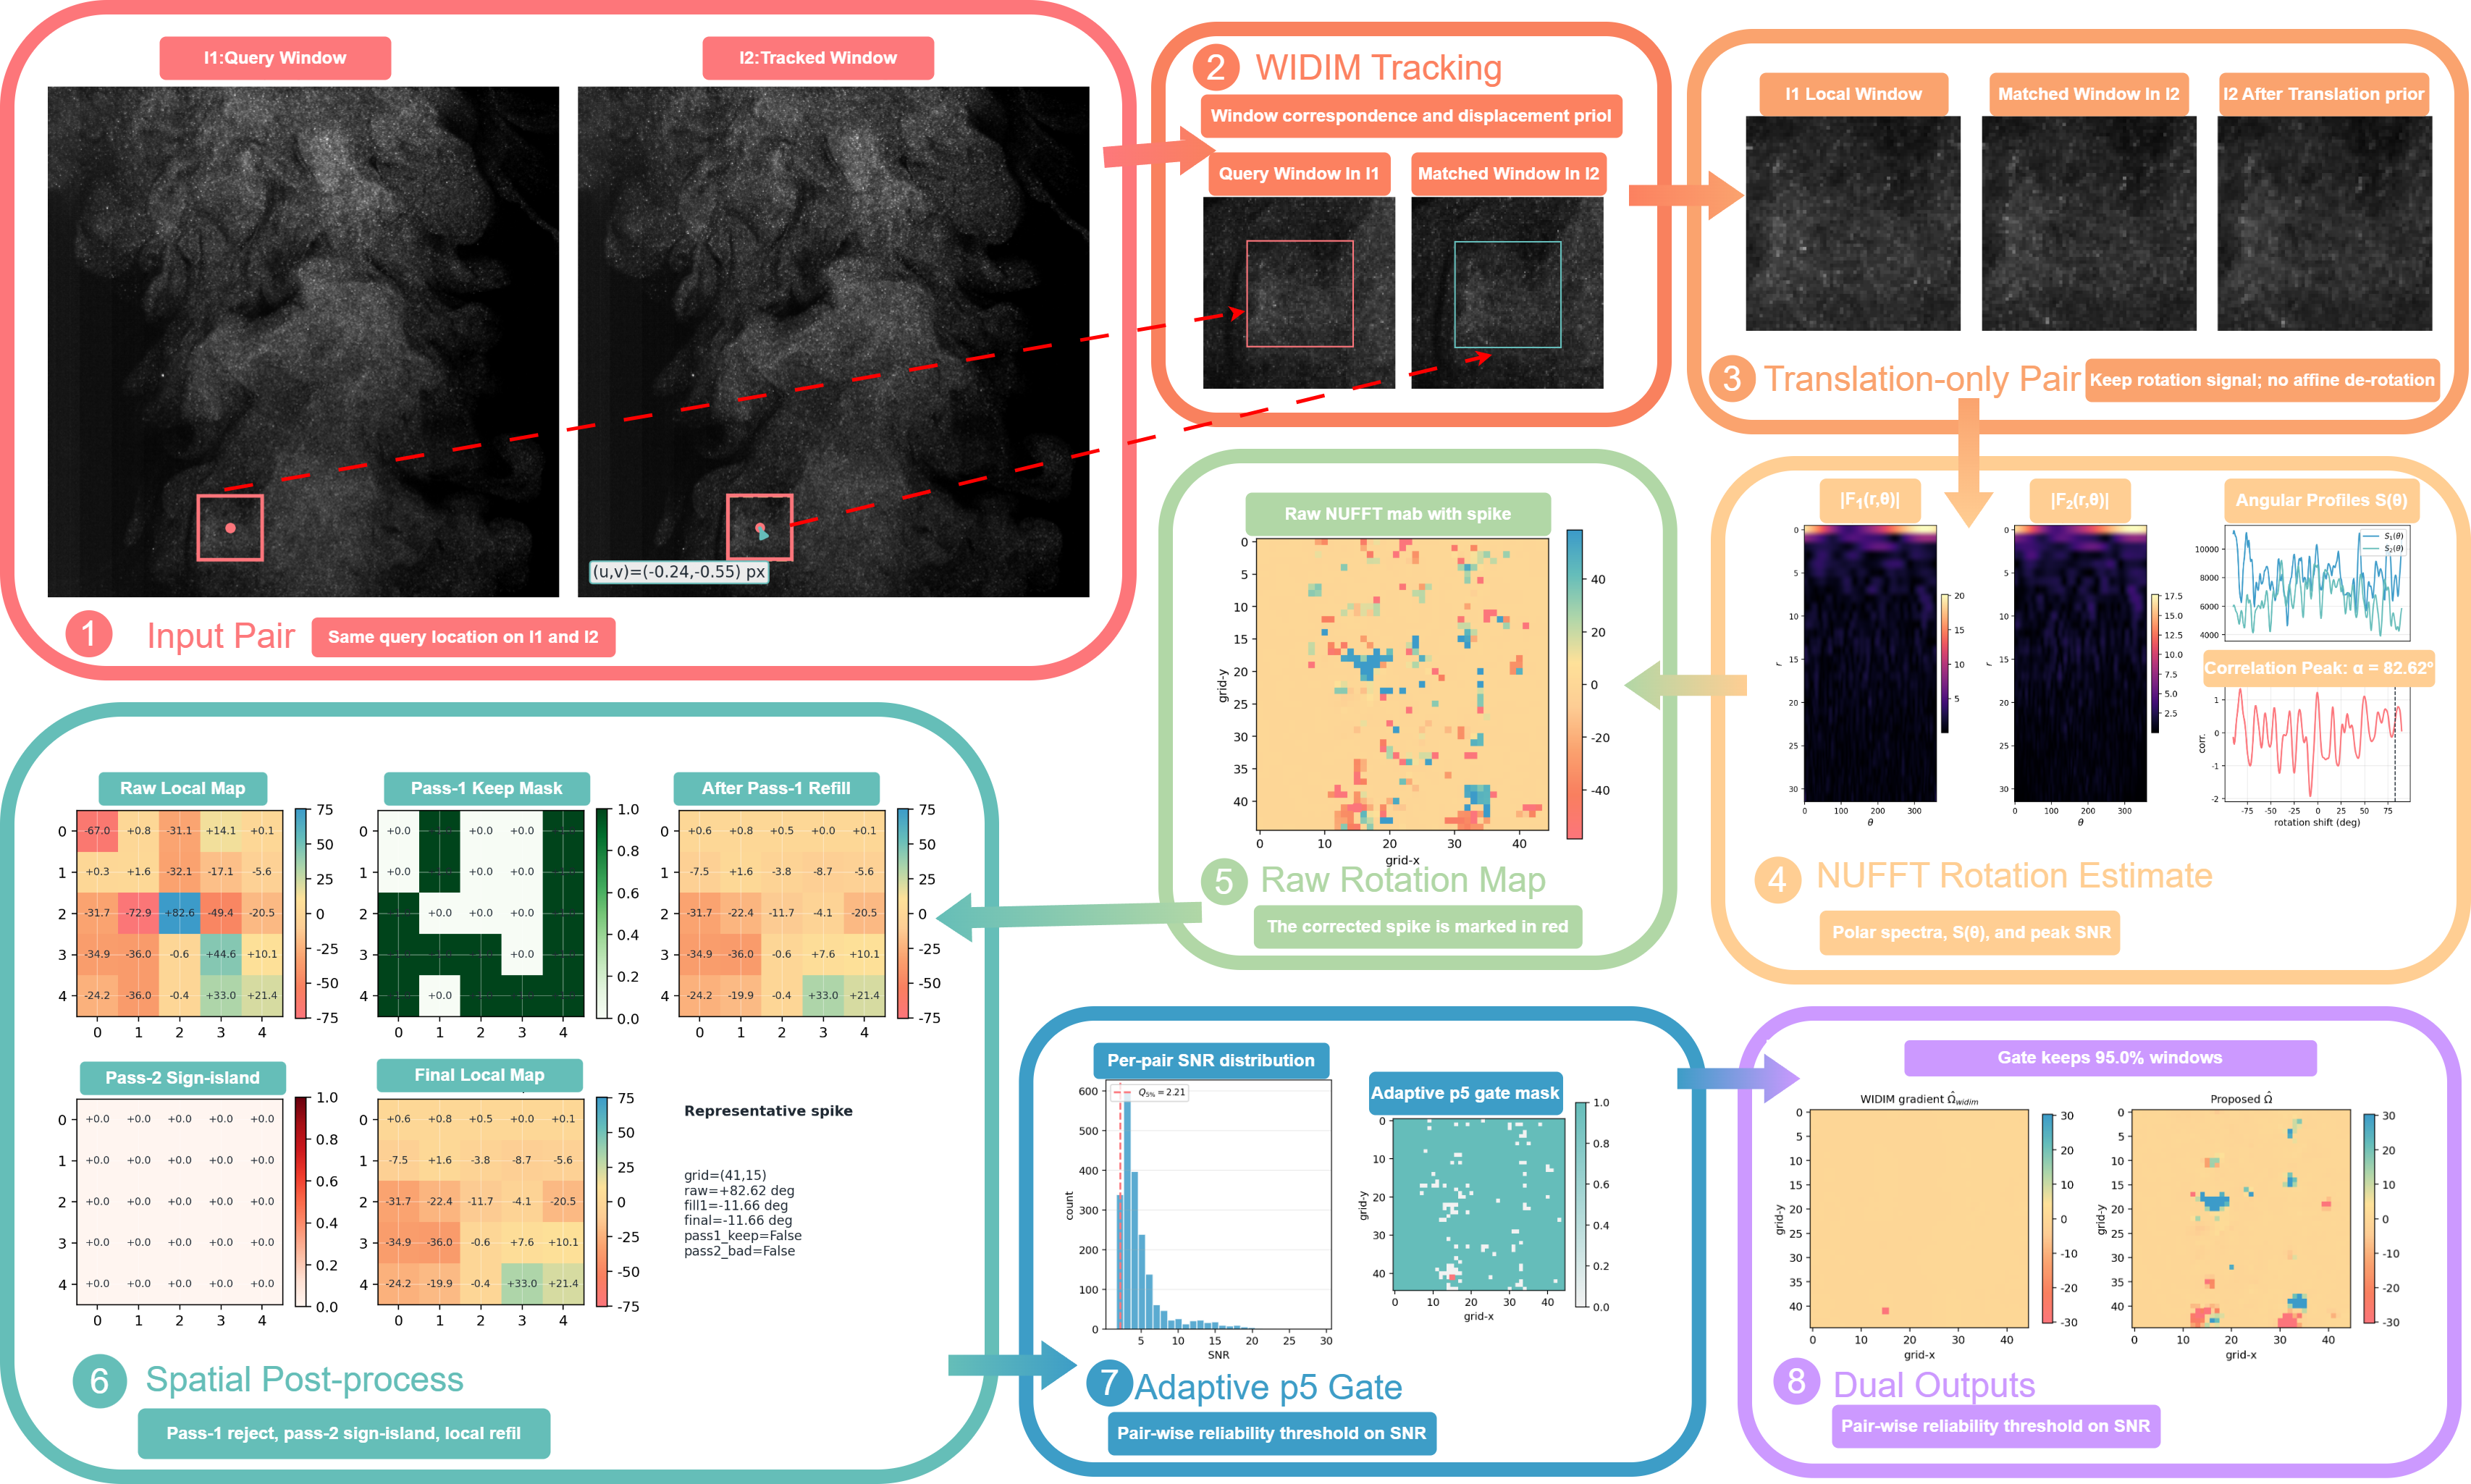
\includegraphics[width=0.98\textwidth]{figures/main/fig01_system_arch.png}
\caption{Workflow of the practical WIDIM(track)+NUFFT protocol on a representative real PIV pair.
    WIDIM supplies window tracking and translation priors, NUFFT estimates the local rotation from polar-spectrum correlation, and two-stage post-processing with adaptive p5 gating controls reliability before the final WIDIM-reference and proposed rotation-rate outputs are produced.}
  \label{fig:system_arch}
\end{figure*}

Prior work relevant to the present study falls into three broad groups.
One direction concerns the accuracy and uncertainty of displacement estimation itself.
Westerweel~\cite{Westerweel1997} and Sciacchitano~\cite{Sciacchitano2019}
systematically summarized cross-correlation-based displacement estimation,
its error sources,
and uncertainty-quantification frameworks.
More recent work has continued toward local uncertainty indicators and gradient-sensitive scenarios,
including pointwise error estimation based on synthetic tests and correlation-plane metrics~\cite{Novotny2025LPR},
surrogate-assisted cross-correlation refinement~\cite{Lee2024},
as well as velocity-field correction and wall-shear-stress recovery in near-wall or boundary measurements~\cite{Walbecq2024Boundary,Willert2025WSS}.
Together, these studies show that PIV can continue to improve at the displacement-field level,
yet once the target becomes a derived quantity such as wall gradients, shear, or rotational structure,
error propagation and local structural distortion become more sensitive than displacement estimation itself.

Another direction concerns frequency-domain registration and rotation-correction tools.
Spectral shift estimation, phase correlation, and rotation correction~\cite{Tong2019,Guizar2008,Nie2023RotationCorrection}
provide mature spectral operators for local angular analysis,
but they have mostly been used for registration, correction, or global angle recovery.
They do not recast local PIV rotation-rate measurement itself as an independent estimation target.

A third direction is the rapidly growing literature on learning-based PIV.
Recent methods have progressed from recurrent optical flow, image preprocessing, and unsupervised reconstruction
to Transformer-driven velocity-field estimation, lightweight flow models, spatial refinement strategies, and stereo deployment
~\cite{Lagemann2022Generalization,Fan2023PIVPreprocess,Shan2024PIVOpticalFlow,Yu2024AttentionalPIV,Reddy2025TwinsPIVNet,Shan2025Lightweight,Choi2023SpatialRefinement,Elrefaie2024StereoPIV,Ji2024,Prakosa2025,Huettig2024,Cai2024},
substantially improving displacement estimation, image quality, and multi-view velocity reconstruction.
Their outputs are still primarily displacement or velocity fields.
They do not bypass the uncertainty propagation induced by differentiating displacement to obtain rotation rate,
nor do they establish a CRLB framework that treats the local rotation angle or rotation rate as the direct measurement target.

The CRLB characterizes the optimal achievable precision of unbiased estimators~\cite{Kay1993}.
Westerweel~\cite{Westerweel1997} provided a CRLB approximation for cross-correlation-based displacement estimation,
and Sciacchitano~\cite{Sciacchitano2019} reviewed uncertainty quantification in PIV.
For local rotation rate, the CRLB theory remains incomplete.
Existing work usually treats rotation rate as a derivative of displacement,
rarely formulates a Fisher-information framework that directly targets the local rotation angle or rotation rate,
and has not quantified the structural precision loss of the gradient path relative to an information-theoretic bound.

The key question is whether local rotation rate can be estimated directly from spectral angular shift rather than inferred by finite differencing of an estimated displacement field.
The theoretical object is a NUFFT-based direct estimator,
and the practical contribution is its minimal deployable form under finite-window PIV,
namely WIDIM(track)-based translation priors together with percentile-based reliability control.

The contributions are threefold.
First, it establishes a CRLB framework that directly targets the local rotation angle and rotation rate, derives the 2D bound, the 1D information-reduction relationship, and an accurate practical weighting approximation, and quantifies the structural precision limitation of the WIDIM gradient path.
Second, it develops a direct rotation-rate estimator on the NUFFT polar magnitude spectrum and deploys it as WIDIM(track)+NUFFT with percentile-based reliability control. Under the final Rankine protocol, this pipeline reduces the RMSE from $1.102^\circ$ to $0.864^\circ$ ($1.28\times$, or $21.6\%$, Monte Carlo $N=12000$).
Third, through ideal uniform rotation, the primary Rankine experiment, multi-flow ground-truth comparisons, a displacement-orthogonality check, and calibrated real-data studies, it delineates the applicability boundary of the direct measurement path and distinguishes precision gain from structural recovery.

\section{Methodology}
\label{sec:theory}
% ------------------------------------------------------------------

The CRLB and observation model for direct local rotation-rate estimation in PIV are developed first, followed by the minimal deployable protocol used under practical finite-window conditions.
In that protocol, WIDIM(track) provides displacement priors only,
while gating and refill act only as reliability-control mechanisms and do not alter the direct measurement object itself.
The displacement CRLB is retained only as a reference bound for the displacement path
to indicate the operating regime of the WIDIM branch.
Its numerical validation and auxiliary figures are collected in the supplementary sections
``Displacement-Path Reference Bound''
and
``Additional Theoretical Diagnostics'',
rather than treated as a second theory line parallel to the rotation-rate CRLB.
Figure~\ref{fig:system_arch} summarizes the full workflow of the final deployable protocol on a real PIV image pair.

%------------------------------------------------------------------
\subsection{Structural Limitation of Finite-Difference Rotation Rate}
\label{sec:widim_limit}
%------------------------------------------------------------------

WIDIM~\cite{Scarano2000} solves the displacement field through iterative affine window deformation,
and its displacement estimation can reach a Cram\'{e}r--Rao efficiency of approximately $\eta_{\rm disp} \approx 34\%$.
In standard PIV practice, the local rotation rate is still extracted from the displacement field by finite differencing:
%
\begin{equation}
  \hat{\Omega}_{\rm WIDIM}(x,y)
  = \frac{1}{2}\!\left(\frac{\partial \hat{v}}{\partial x}
    - \frac{\partial \hat{u}}{\partial y}\right),
  \label{eq:omega_widim}
\end{equation}
%
where $(\hat{u}, \hat{v})$ are the displacement components estimated by WIDIM.
If the displacement errors on the four-point central-difference stencil are approximately independent and homoscedastic with standard deviation $\sigma_d$,
then the propagated uncertainty of the local rotation rate defined by~\eqref{eq:omega_widim} becomes
%
\begin{equation}
  \sigma_{\Omega,\rm WIDIM}
  = \frac{\sigma_d}{2\Delta x}\quad [\mathrm{rad/frame}]
  = \frac{180}{\pi}\frac{\sigma_d}{2\Delta x}\quad [^\circ\!/\mathrm{frame}].
  \label{eq:sigma_omega}
\end{equation}
%
Under the representative setting used here,
$\sigma_d=0.18\,$px and $\Delta x=32\,$px,
Eq.~(\ref{eq:sigma_omega}) yields
$\sigma_{\Omega,\rm WIDIM}\approx 0.161\,^\circ\!/\mathrm{frame}$.
The uncertainty of the gradient path with respect to $\Omega$ propagates as $O(\sigma_d/\Delta x)$.
The limitation is structural:
even when displacement estimation itself approaches the CRLB,
rotation-rate estimation must still absorb the information loss introduced by spatial differencing.
To alleviate this measurement bottleneck, one must introduce a direct rotation-rate estimator that does not rely on differentiating the displacement field.

%------------------------------------------------------------------
\subsection{Cram\'{e}r--Rao Bound for Rotation Estimation}
\label{sec:crlb_rotation}
%------------------------------------------------------------------

\subsubsection{Observation Model}

Let the Fourier magnitude spectra of the reference window $W_1$ and target window $W_2$ be
$|F_1|$ and $|F_2|$, respectively.
By the Fourier shift theorem, translation affects only the phase and does not change the magnitude spectrum.
Hence the local rotation angle $\alpha$ can be estimated independently from magnitude information.
The observation model on the polar grid $(r_j,\theta_k)$ is
%
\begin{equation}
  M_{jk} = A(r_j,\, \theta_k - \alpha) + n_{jk},
  \label{eq:obs_model}
\end{equation}
%
where $A(r,\theta) \triangleq |F_1(r,\theta)|$ is the reference magnitude spectrum,
$\alpha$ is the unknown rotation angle,
and $n_{jk} \sim \mathcal{N}(0,\sigma^2)$ denotes independent Gaussian noise.
Under the high-SNR approximation, $\sigma^2 \approx N^2 \sigma_s^2 / 2$,
where $N$ is the window size and $\sigma_s$ is the standard deviation of the spatial-domain image noise.

\subsubsection{2D Fisher Information and the Exact Bound}

Result 1 (2D Fisher information):
under the observation model~\eqref{eq:obs_model}, the Fisher information of the rotation angle $\alpha$ is
%
\begin{equation}
  \mathcal{I}_{2D}
  = \sum_{j \geq j_{\min}} \sum_{k=1}^{N_\theta}
    \frac{[\partial A(r_j, \theta_k)/\partial\theta]^2}{\sigma^2},
  \label{eq:fisher_2d}
\end{equation}
%
where the summation is restricted to $r_j \geq r_{\min}$ so as to exclude the low-SNR low-frequency region.
By the Cram\'{e}r--Rao theorem, any unbiased estimator $\hat{\alpha}$ satisfies
%
\begin{equation}
  \Var(\hat{\alpha}) \geq \CRLB_{2D}
  = \frac{1}{\mathcal{I}_{2D}}.
  \label{eq:crlb_2d}
\end{equation}
%
A representative numerical value is $\CRLB_{2D}^{1/2} \approx 0.018^\circ$
for $\sigma_s = 0.01$ and $N=64\,\mathrm{px}$.

\subsubsection{Information Reduction from 2D to 1D}

In the practical algorithm, the magnitude spectrum is compressed into a one-dimensional angular feature by weighted radial integration:
%
\begin{equation}
  S_W(\theta_k) = \sum_{j \geq j_{\min}} W(r_j)\,|F(r_j, \theta_k)|,
  \label{eq:radial_int}
\end{equation}
%
where $W(r)$ is the radial weighting function.
This dimensionality reduction introduces information loss.

Result 2 (information-loss inequality):
for any nonzero weighting function $W(r)$, the lower bound achievable by the radially integrated estimator satisfies
%
\begin{equation}
  \CRLB_{1D}(W) \geq \CRLB_{2D},
  \label{eq:hierarchy}
\end{equation}
%
with equality if and only if $W(r_j) \propto g(r_j)/\sigma^2(r_j)$,
where $g(r_j)$ denotes the RMS angular gradient at radius $r_j$,
and the proportionality is consistent across all angles $\theta_k$.

\textit{Sketch of derivation:}
the Fisher information of $S_W(\theta_k)$ can be written as
$\mathcal{I}_{1D} = \|\bfM\bfw\|^2 / (\sigma^2\|\bfw\|^2)$,
where $\bfw = (W_1,\ldots,W_{N_r})^T$
and $\bfM$ is the angular-gradient matrix.
By the Cauchy--Schwarz inequality,
$\mathcal{I}_{1D} \leq \mathcal{I}_{2D}$,
and taking reciprocals yields~\eqref{eq:hierarchy}.
\subsubsection{Optimal Radial Weighting}
Result 3 (optimal weighting):
maximizing $\mathcal{I}_{1D}$ is equivalent to solving the generalized Rayleigh quotient
%
\begin{equation}
  W^* = \mathop{\arg\max}_{\bfw \neq 0}
  \frac{\bfw^T \bfM \bfw}{\bfw^T \bfw},
  \label{eq:optimal_weight}
\end{equation}
%
where the entries of the angular-gradient covariance matrix $\bfM$ are
$M_{jj'} = \sum_k \dot{A}(r_j,\theta_k)\dot{A}(r_{j'},\theta_k)$,
$\dot{A} = \partial A/\partial\theta$.
The optimal weighting $W^*$ is the principal eigenvector of $\bfM$ associated with its largest eigenvalue.

Numerical Observation 1 ($r^2$ approximation):
for PIV speckle-like particle images, the power spectrum approximately decays as $|F(r,\theta)|^2 \propto r^{-4}$.
Under the separable approximation $\dot{A}(r,\theta) \approx g(r)h(\theta)$,
the Pearson correlation between $W^*(r)$ and $r^2$ is 0.80 (numerical validation is provided in Section~\ref{sec:exp_crlb}).
Using $W(r)=r^2$ as a practical approximation to the optimal weighting
reaches about $80\%$ CRLB efficiency in the controlled uniform-rotation regime.

\subsubsection{Metric Convention and Representative Scale}

In the ideal uniform-rotation setting, NUFFT efficiency is reported against $\CRLB_{1D}$ as the theoretical reference.
For translation-bearing synthetic flows, by contrast, the main comparison metrics are RMSE, confidence intervals, and relative improvement factors.
This convention is used consistently throughout the remainder of the paper:
ideal uniform rotation serves only for theoretical-efficiency validation,
whereas the final Rankine and multi-flow experiments are compared primarily by RMSE, confidence intervals, and relative gain.

%------------------------------------------------------------------
% ------------------------------------------------------------------
\subsection{NUFFT-Based Direct Rotation-Rate Estimation}
\label{sec:method}
% ------------------------------------------------------------------

Based on the CRLB theory above (Eqs.~\eqref{eq:crlb_2d}--\eqref{eq:optimal_weight}), the direct rotation-rate estimator is implemented on the NUFFT polar magnitude spectrum.
The estimator outputs the inter-frame local rotation angle $\hat{\alpha}$;
for a time interval $\Delta t$, the corresponding rotation rate is
$\hat{\Omega}=\hat{\alpha}/\Delta t$.
All experiments use $\Delta t=1$ frame,
so the numerical values are reported directly in $^\circ/\mathrm{frame}$.
The observation object and solution pipeline are described first, followed by deployment under finite-window PIV conditions.
The direct estimator relies on two basic properties of the Fourier magnitude spectrum.
The first is shift invariance:
for any square-integrable function $f$,
\begin{equation}
  \bigl|F\bigl\{f(x-t)\bigr\}(k)\bigr|
  = \bigl|F\{f(x)\}(k)\bigr|,
  \label{eq:shift_invariance}
\end{equation}
which holds exactly on an infinite domain~\cite{Tong2019,Guizar2008}
and implies that the magnitude spectrum does not carry translation information.
The second is rotation equivariance:
if $f_2(x)=f_1(R_\alpha x)$,
then the polar magnitude spectra satisfy~\cite{Tong2019,Guizar2008}
\begin{equation}
  |F_2(r,\theta)| = |F_1(r,\,\theta - \alpha)|,
  \label{eq:rotation_equivariance}
\end{equation}
That is, a spatial rotation by $\alpha$ becomes an angular shift by $\alpha$ on the polar magnitude spectrum.
Together, these two properties convert local rotation estimation into a one-dimensional cyclic peak-localization problem in polar space.

In practical PIV, finite windows violate the infinite-domain assumption.
Mean removal and Hanning windowing are applied to each local patch to reduce spectral leakage induced by truncation.
Under this treatment, the shift invariance of the magnitude spectrum remains sufficiently accurate on local speckle windows to support direct rotation-rate estimation.
On the numerical side, evaluating the polar magnitude spectrum $|F(r,\theta)|$ requires sampling the Cartesian spectrum at nonuniform polar locations.
Conventional interpolation introduces systematic bias in the high-frequency region~\cite{Press2007},
which can dominate rotation-estimation error in the low-noise regime.
NUFFT~\cite{Barnett2019,Barnett2021} is used
to compute the spectrum directly at the polar frequency points with near machine precision,
thereby avoiding interpolation bias as an artificial limiter of the estimator's achievable precision.

%------------------------------------------------------------------
\subsection{Algorithmic Procedure}
\label{sec:algorithm}
%------------------------------------------------------------------

The core idea of the algorithm is to exploit the shift invariance of the Fourier magnitude spectrum
to decouple rotation from translation,
and then use rotation equivariance---namely, that a spatial rotation $\alpha$ becomes an angular shift $\alpha$ on the polar magnitude spectrum---to estimate the local rotation angle directly via one-dimensional cyclic correlation in polar space.

The full procedure is summarized in Algorithm~\ref{alg:nufft_rotation}.

\begin{algorithm}
\caption{NUFFT Polar-Magnitude Rotation-Rate Estimation}
\label{alg:nufft_rotation}
\begin{algorithmic}[1]
  \REQUIRE Window pair $(W_1, W_2)$ and parameters $N_r, N_\theta, r_{\min}, \varepsilon$
  \ENSURE Rotation-angle estimate $\hat{\alpha}$, rotation rate $\hat{\Omega}$, and SNR

  \STATE Preprocess: mean removal + Hanning window
    $\rightarrow W_i' = (W_i - \bar{W}_i) \cdot h_{\rm Hann}$
  \STATE FFT: $F_i = \mathrm{FFT2}(W_i')$ and keep the magnitude spectrum $|F_i|$
  \STATE NUFFT polar sampling: evaluate the spectrum on grid points
    $(r_j, \theta_k),\; j=1,\ldots,N_r,\; k=1,\ldots,N_\theta$
    to obtain $\tilde{F}_i(r_j, \theta_k)$ with interpolation-equivalent error $< \varepsilon = 10^{-9}$
  \STATE Radial integration:
    $S_i(\theta_k) = \sum_{r_j \geq r_{\min}} r_j^2 \cdot |\tilde{F}_i(r_j, \theta_k)|$
  \STATE Circular cross-correlation:
    $C(\delta) = \sum_k S_1(\theta_k) \cdot S_2(\theta_k + \delta)$
  \STATE Subpixel peak fitting: three-point Gaussian interpolation
    $\rightarrow \hat{\alpha}_{\rm raw}$, SNR $= C_{\max}/C_{\rm sidelobe}$
  \STATE Two-stage post-process:
    \STATE Stage 1: spatial-consistency screening (z-score / gradient / Laplacian)
      with an additional weak-SNR large-angle rejection rule
    \STATE Stage 2: sign-island rejection with locally bounded refill, yielding $\hat{\alpha}_{\rm new}$
  \STATE Adaptive gating: compute $p5(\mathrm{SNR})$ from the SNR distribution of the current image pair
    and retain only windows with $\mathrm{SNR} \ge p5$ for statistics
  \STATE Output $\hat{\alpha}_{\rm raw},\hat{\alpha}_{\rm new}$ and the gated mask
  \RETURN $\hat{\Omega}_{\rm raw},\hat{\Omega}_{\rm new}$, SNR
\end{algorithmic}
\end{algorithm}

In Step~3, NUFFT polar sampling maps the FFT result from the Cartesian frequency grid to the polar grid:
%
\begin{align}
  (s_x, s_y) &= \bigl(r_j \cos\theta_k,\; r_j \sin\theta_k\bigr), \\
  \tilde{F}(r_j, \theta_k) &= \sum_{m,n} F_{mn}\,
    e^{-2\pi i (s_x m + s_y n)/N}.
  \label{eq:nufft}
\end{align}
%
The computational complexity of the NUFFT stage is
$O(N^2 \log N + N_r N_\theta \log(1/\varepsilon))$,
which is of the same asymptotic order as interpolation-based implementations and does not introduce an additional order-of-magnitude complexity penalty.

%------------------------------------------------------------------
\subsection{Physical Rationale for the Key Parameters}
\label{sec:params}
%------------------------------------------------------------------

Interpolation tolerance $\varepsilon = 10^{-9}$ keeps numerical sampling error well below image-noise-induced spectral noise and suppresses the high-frequency bias of conventional interpolation. The minimum radius $r_{\min}=8\,\mathrm{px}^{-1}$ removes the nearly isotropic low-frequency band whose Fisher-information contribution is negligible. Parameter sweeps over $r_{\min}\in[6,10]$ change the RMSE by less than $3\%$. The practical weighting $W(r)=r^2$ approximates $W^*(r)$ with correlation $0.80$ and yields about $80\%$ CRLB efficiency in controlled experiments. Adaptive p5 gating computes the threshold from each pair-specific SNR distribution and suppresses long-tail contamination without introducing the cross-domain bias of a fixed absolute threshold.

%------------------------------------------------------------------
\subsection{Computational Complexity}
\label{sec:complexity}
The computational order of the direct estimator remains $O(N^2\log N + N_rN_\theta)$, matching interpolation-based implementations in asymptotic order. Measured runtime differs by only about $0.99\times$ over window sizes from $64$ to $512\,$px. Detailed complexity breakdowns are reported in the supplement.

%------------------------------------------------------------------
\subsection{Deployable Protocol for Practical PIV}
\label{sec:system}
%------------------------------------------------------------------

The NUFFT direct estimator defined above is the theoretical object of the paper.
In practical PIV, finite windows, particle turnover, and local translation can weaken direct spectral matching.
The deployable protocol preserves the same measurement object while adding only WIDIM(track)-based displacement priors and reliability control at the input side:
WIDIM(track) maintains window correspondence,
NUFFT performs direct rotation-rate estimation,
and the two-stage post-process together with percentile gating serves only for reliability control.
Figure~\ref{fig:system_arch} summarizes the stage-by-stage workflow of the system.
the focus here is its physical division of labor and deployment constraints.
Further arguments for translation-only alignment and adaptive percentile gating are given in the supplementary section
``Additional Rationale for Deployment-Side Design Choices''.

For an input image pair $(I_1, I_2)$, the protocol contains three functional layers:

\begin{itemize}
  \item \textbf{Displacement-prior layer:}
    the WIDIM branch outputs the displacement field $(\hat{u}, \hat{v})$,
    which is used to provide a translation-only window-alignment prior;
    the corresponding displacement efficiency is $\eta_{\rm disp} \approx 34\%$.
  \item \textbf{Direct rotation-rate estimation layer:}
    Algorithm~\ref{alg:nufft_rotation} estimates the local rotation angle $\hat{\alpha}(i,j)$
    independently for the window pair at each spatial location,
    and outputs the local rotation-rate field as $\hat{\Omega}(i,j)=\hat{\alpha}(i,j)/\Delta t$;
    throughout the paper $\Delta t=1$ frame, so the numerical values are reported directly in $^\circ/\mathrm{frame}$;
    under controlled rotation, the efficiency is $\eta_{\rm rot} \approx 80\%$.
  \item \textbf{Reliability-control layer:}
    a two-stage post-process (spatial gating + sign-island rejection and refill) is used,
    followed by Adaptive p5 gating on the statistical side to unify the evaluation protocol across synthetic and real data.
\end{itemize}

The deployable protocol preserves two constraints:
WIDIM provides only the displacement prior and displacement output,
and NUFFT operates only on the translation-aligned raw window pair without using displacement gradients.
The two output branches remain physically orthogonal.
Empirically, the displacement RMSE of WIDIM+NUFFT differs from standalone WIDIM by only $+0.04\%$.

\subsection{Three Design Constraints for Direct Rotation-Rate Estimation in Practical PIV}
\label{sec:evolution_reason}

A controlled V0--V3 ablation is used to isolate the constraints that practical direct rotation-rate estimation must satisfy.
Window size, step size, noise level, NUFFT sampling parameters, and the evaluation protocol are held fixed, and each variant changes only one design choice.
The three constraints are maintaining window correspondence, preserving the rotation signal, and suppressing low-confidence outliers.

The first constraint is \textbf{maintaining window correspondence}.
Particle turnover weakens the correspondence between two local windows.
For a window size $N$ and inter-frame displacement magnitude $|d|$, the particle-loss rate is approximately
%
\begin{equation}
  F_{\rm loss} \approx \frac{|d|}{N},
  \label{eq:evo_loss}
\end{equation}
%
As a result, the fixed-window NUFFT baseline (V0) becomes prone to window mismatch and peak degradation under translation-bearing PIV conditions,
showing that the direct estimator requires a displacement prior to maintain window correspondence in practice.

The second constraint is \textbf{preserving the rotation signal}.
V1 introduces WIDIM affine windows on top of V0 to alleviate mismatch,
but the affine matrix itself contains a rotational component:
%
\begin{equation}
  \mathbf{T}_{\rm affine} =
  \begin{pmatrix}
    \partial \hat{u}/\partial x & \partial \hat{u}/\partial y \\
    \partial \hat{v}/\partial x & \partial \hat{v}/\partial y
  \end{pmatrix},
  \quad
  \Omega_{\rm aff} = \frac{1}{2}\!\left(\frac{\partial \hat{v}}{\partial x}
  - \frac{\partial \hat{u}}{\partial y}\right),
  \label{eq:evo_affine}
\end{equation}
%
Affine preconditioning can partially cancel the very rotation signal that NUFFT is intended to estimate.
V2 switches to a ``track-prior only'' windowing strategy,
which minimizes registration error while preserving the rotational content.

The third constraint is \textbf{suppressing low-confidence outliers}.
Even when window correspondence is maintained, low-confidence windows may still produce isolated spikes
that dominate the statistics through the tail of the error distribution.
V3 adds a two-stage post-process and adaptive percentile gating on top of V2,
specifically to suppress the statistical dominance of such outliers.
At the statistical stage, only windows satisfying
%
\begin{equation}
  \mathrm{SNR}_{ij} \geq Q_{5\%}\!\left(\{\mathrm{SNR}\}_{\text{pair}}\right),
  \label{eq:evo_p5}
\end{equation}
%
and combines this rule with spatial rejection and refill to suppress isolated spikes.
The controlled V0--V3 comparison shows that
WIDIM is responsible only for maintaining window correspondence and providing a translation prior,
NUFFT is responsible for direct rotation-rate estimation,
and percentile-based reliability control is responsible only for suppressing low-confidence outliers,
without altering the measurement object of the direct estimator.
These three constraints define the design target of V3,
while its final adoption is supported jointly by qualitative evidence and cross-scenario quantitative results.

\begin{figure}[!htbp]
  \centering
  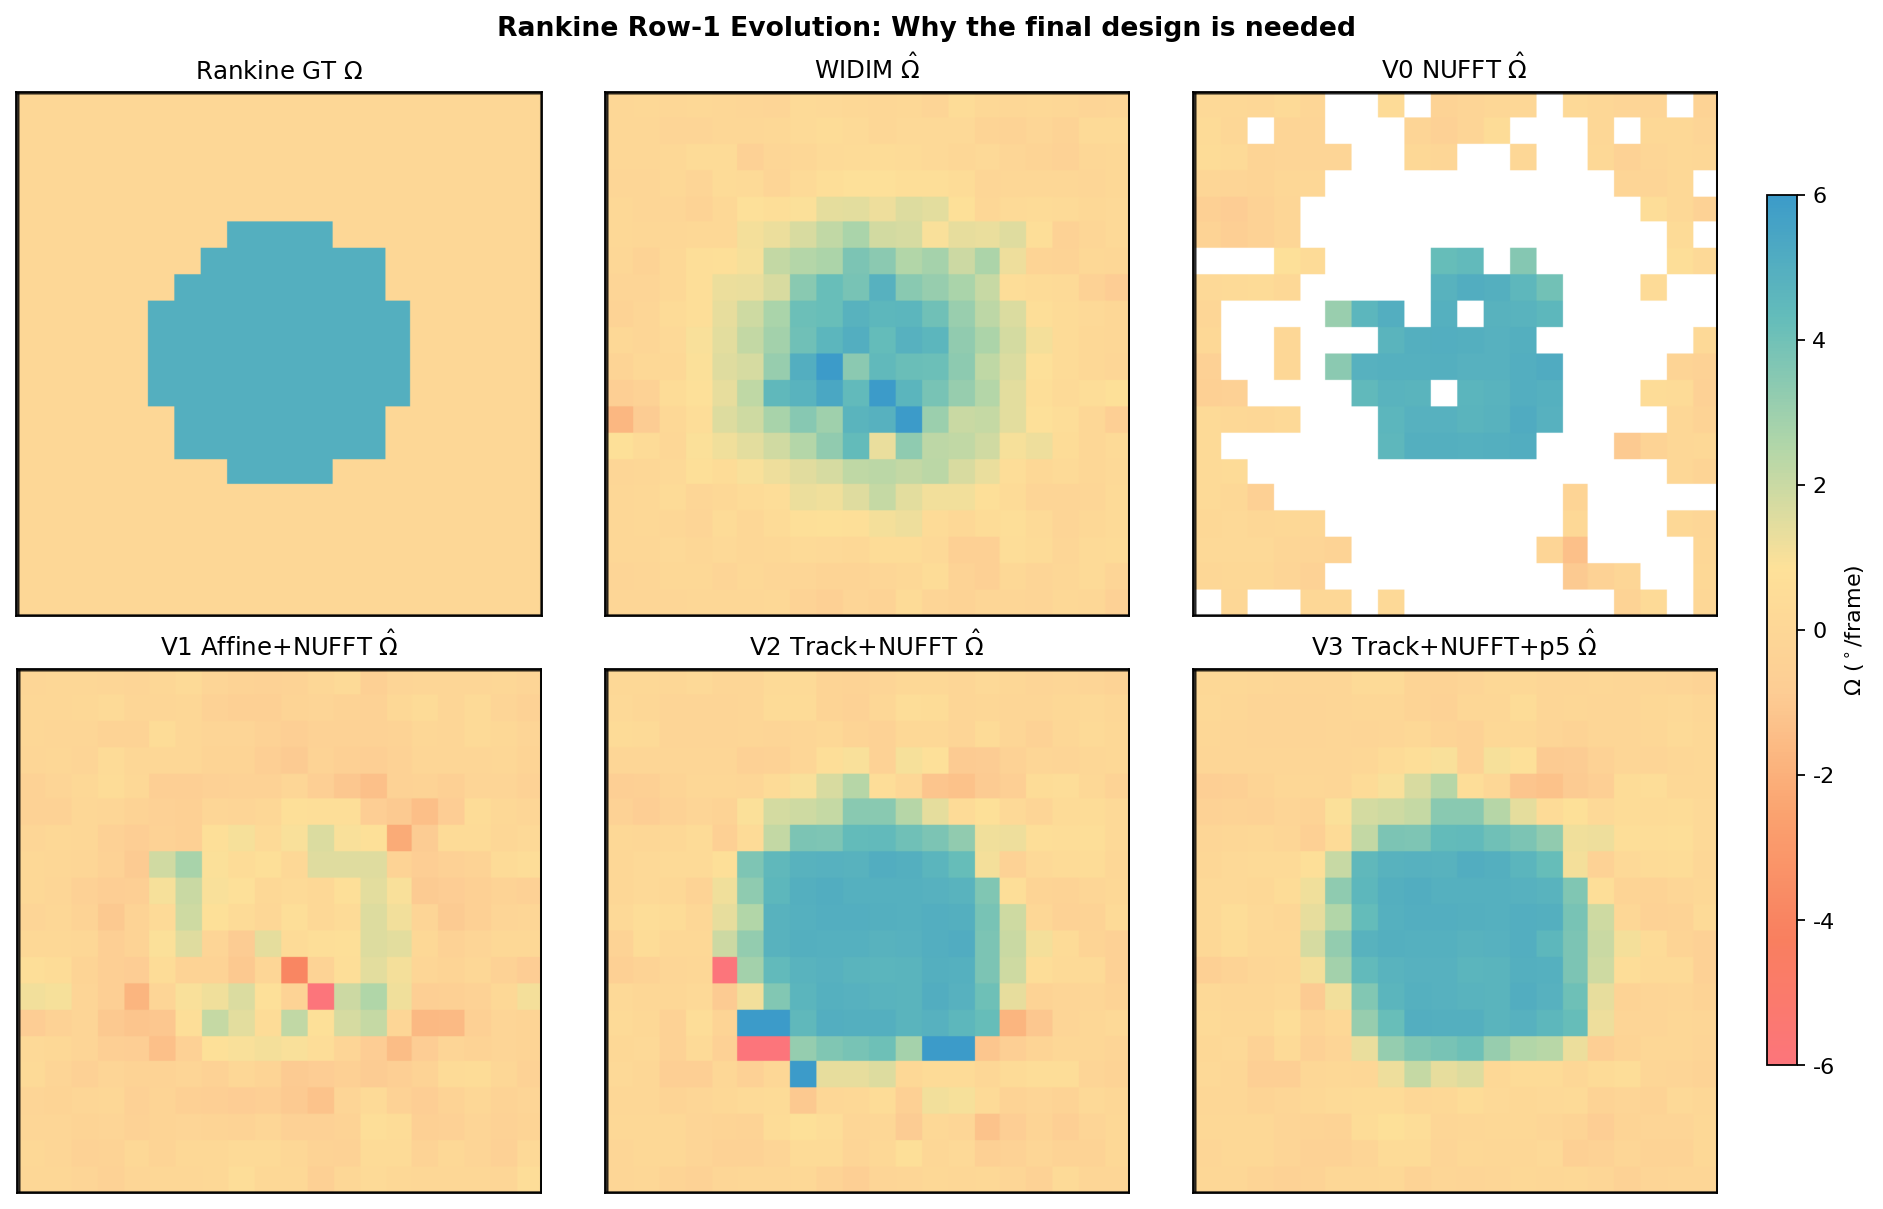
\includegraphics[width=\columnwidth]{figures/main/fig02_rankine_evolution.png}
\caption{Controlled ablation in the Rankine setting under identical window, noise,
  and sampling conditions.
  V0$\rightarrow$V3 isolates the effect of each design change on the same case.}
  \label{fig:pipeline_evolution_rankine}
\end{figure}

Figure~\ref{fig:pipeline_evolution_rankine} provides the qualitative evidence on a single Rankine case:
V0 yields the lowest error only under the idealized fixed-window condition,
V1 weakens the target rotational signal through affine preprocessing,
and V2 preserves the signal but still lacks a mechanism to suppress low-confidence outliers.
A single case is insufficient to select the final protocol.
Figure~\ref{fig:gt_summary} summarizes the paired RMSE ratios across four synthetic flows.
The summary shows that different protocol variants can be favorable in different scenarios,
whereas V3 is the most robust in the geometric-mean sense across flows.
V3 is adopted as the final deployable protocol used throughout.

\begin{figure}[!htbp]
  \centering
  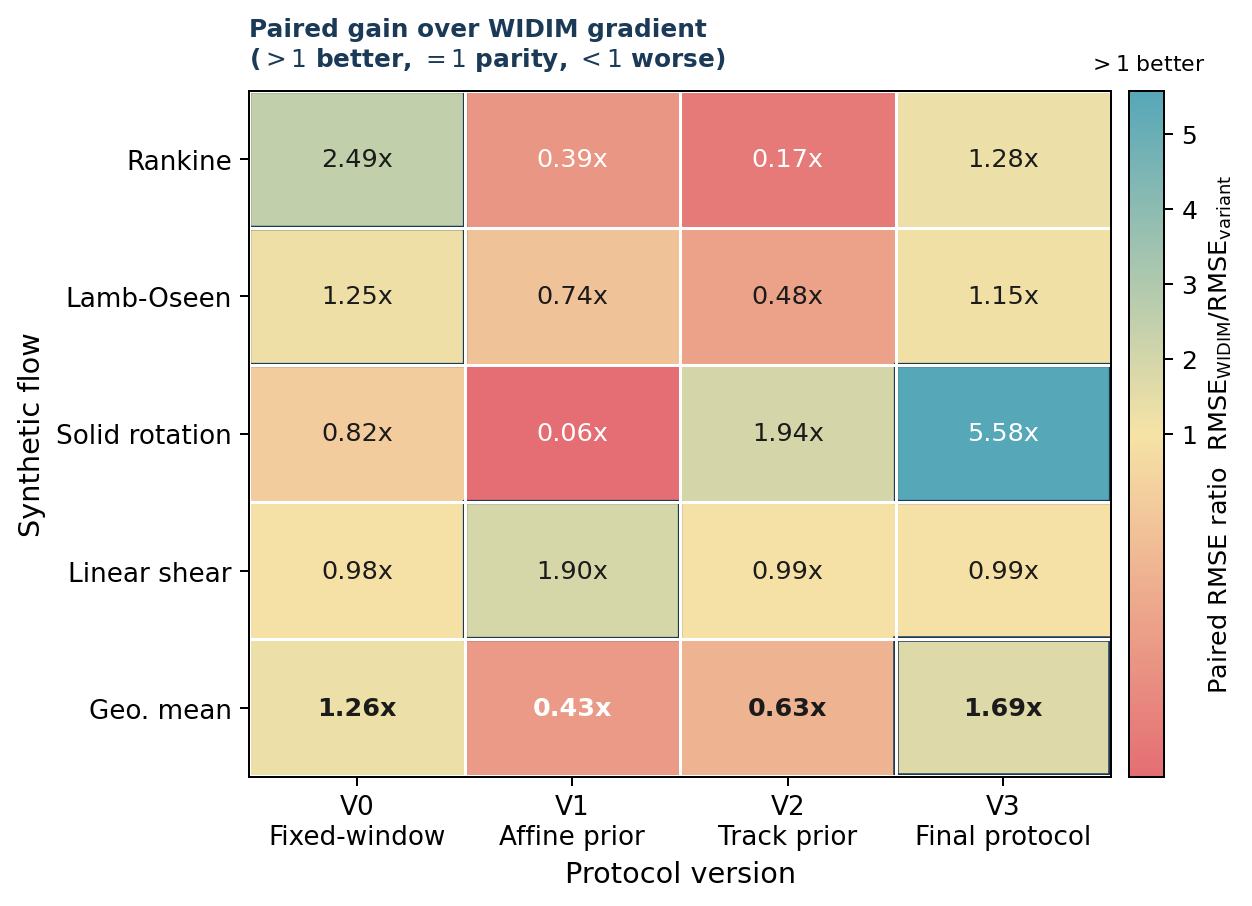
\includegraphics[width=\columnwidth]{figures/main/fig03_protocol_summary.png}
  \caption{Protocol summary across four synthetic flows.
    Each cell reports $\mathrm{RMSE}_{\mathrm{WIDIM}}/\mathrm{RMSE}_{\mathrm{variant}}$
    ($>1$ better; $1$ parity; $<1$ worse).
    V0 is strongest under the idealized fixed-window Rankine setting,
    whereas V3 achieves the best geometric-mean gain across flows.}
  \label{fig:gt_summary}
\end{figure}

The default implementation parameters of the final protocol are reported in the supplement section ``Implementation Details and Default Parameters''.

% ------------------------------------------------------------------
\section{Experimental Setup and Quantitative Analysis}
\label{sec:synthetic}
% ------------------------------------------------------------------

Experiments are organized from ideal validation to real-data deployment.
After CRLB validation under uniform rotation, the Rankine vortex serves as the \textbf{primary validation experiment} for the deployable protocol.
Multi-flow ground-truth comparisons delineate the applicability boundary.
A displacement-orthogonality test and a real-data study then verify, respectively, that the integrated system does not damage the WIDIM displacement branch and that real-data results are interpreted as calibrated proxy evidence rather than direct absolute-accuracy claims.

%------------------------------------------------------------------
\subsection{Numerical Validation of CRLB Efficiency}
\label{sec:exp_crlb}
%------------------------------------------------------------------

\subsubsection*{Validation of the Rotation-CRLB Hierarchy}

Using a synthetic speckle reference image ($N=64\,$px, $ppp=0.04$, $d_\tau=2.5\,$px, $\sigma_s=0.01$, seed=42), the reference magnitude spectrum $A(r,\theta)=|F_1(r,\theta)|$ and its angular gradient $\partial A/\partial\theta$ are computed first.
The 2D Fisher information $\mathcal{I}_{2D}$ from~\eqref{eq:fisher_2d} and the reduced 1D Fisher information $\mathcal{I}_{1D}(W)$ from~\eqref{eq:radial_int} are then evaluated under five weighting functions $W(r) \in \{1,\,r,\,r^2,\,r^3,\,W^*\}$.
The optimal weighting $W^*(r)$ is obtained through the eigendecomposition of the gradient covariance matrix $\bfM$ (Result~3).

Figure~\ref{fig:crlb1_hierarchy} reports three groups of validation results:
(a) the hierarchy of $\CRLB_{1D}^{1/2}$ under the five weighting functions versus $\CRLB_{2D}^{1/2}=0.018^\circ$, validating the information inequality;
(b) the radial comparison between the optimal weighting $W^*(r)$ and $r^2$, with Pearson correlation $0.80$, validating Numerical Observation~1;
and (c) the radial cumulative Fisher information, showing that all useful information is contributed by bands above $r_{\min}=8\,$px$^{-1}$.

Together with the controlled uniform-rotation experiment,
Fig.~\ref{fig:crlb1_hierarchy} shows that under high-accuracy polar sampling,
NUFFT rotation estimation can remain close to $\CRLB_{1D}^{1/2}$,
with efficiency $\eta_{\mathrm{NUFFT}}\approx 80\%$.

%------------------------------------------------------------------
\subsection{Rotation-Rate Accuracy Comparison: Rankine-Vortex Validation}
\label{sec:exp_rotation}
%------------------------------------------------------------------

\subsubsection{Experimental Configuration}

The Rankine setting simultaneously contains rotational structure, local translation, finite-window mismatch, and analytically available ground truth,
which makes it the primary validation scenario for the proposed protocol.
The synthetic Rankine vortex uses
$\Gamma=1500\,$px$^2$/frame, $R_{\mathrm{core}}=50\,$px,
an image size of $256\times256\,$px, $ppp=0.04$, $d_\tau=2.5\,$px, and $\sigma_s=0.01$.
The theoretical local rotation rate inside the vortex core is
%
\begin{equation}
  \Omega_{\mathrm{truth}} = \frac{\Gamma}{2\pi R_{\mathrm{core}}^2}
  = \frac{1500}{2\pi\times 50^2}
  \approx 5.471^\circ/\mathrm{frame}.
  \label{eq:rankine_truth}
\end{equation}
%
The interrogation window is $N=64\,$px, with a unified step of $10\,$px,
forming a $20\times20$ window grid on the $256\times256\,$px image.
A two-level statistical protocol is used: seed=42 is reserved for visualization, whereas Monte Carlo aggregation uses $N_{\mathrm{seeds}}=30$ random seeds and yields $N=12000$ valid window samples under the final WIDIM(track)+NUFFT protocol with two-stage spatial screening.

\subsubsection{Field Visualization and Monte Carlo Results}

Figure~\ref{fig:rankine_field_vis} shows the visualization for the seed=42 realization:
the ground-truth field, the NUFFT estimate, the WIDIM-gradient field, and the corresponding error maps.
On the same $20\times20$ scanning grid,
the proposed protocol recovers the Rankine-vortex rotational structure more completely.
In the seed=42 visualization,
the NUFFT absolute-error RMSE is about $0.82^\circ$,
whereas the WIDIM gradient baseline is about $1.18^\circ$.

\subsubsection{Monte Carlo Aggregated Statistics}

Table~\ref{tab:mc_rotation} and Fig.~\ref{fig:rankine_mc}
summarize the core ground-truth metrics.
The NUFFT RMSE is $0.864^\circ$ with a 95\% bootstrap CI of $[0.842,\,0.887]$,
whereas the WIDIM RMSE is $1.102^\circ$ with a 95\% bootstrap CI of $[1.084,\,1.119]$.
The confidence intervals do not overlap,
and the proposed protocol improves over the gradient baseline by $1.28\times$,
corresponding to a $21.6\%$ RMSE reduction.
The calibration relationship between proxy metrics and true improvement in the Rankine setting
is reported separately in Table~\ref{tab:proxy_calibration} and in the supplementary section
``Relationship Between No-Ground-Truth Proxy Metrics and True Improvement''
so that the primary Rankine figure remains focused on its role as the main validation evidence.

\begin{table*}[!htbp]
  \renewcommand{\arraystretch}{1.2}
  \caption{Monte Carlo Aggregation for Rankine Rotation-Rate Estimation
    ($N_{\mathrm{seeds}}=30$, $N=12000$, $\sigma_s=0.01$, step$=10$\,px)}
  \label{tab:mc_rotation}
  \centering
  \begin{threeparttable}
    \begin{tabular}{lccc}
      \toprule
      Method & RMSE ($^\circ$) & 95\% CI & $N$ \\
      \midrule
      WIDIM gradient baseline & 1.102 & $[1.084,\,1.119]$ & 12000 \\
      WIDIM-track+NUFFT final protocol & 0.864 ($21.6\%\downarrow$) & $[0.842,\,0.887]$ & 12000 \\
      \midrule
      Relative gain & \multicolumn{2}{c}{$1.28\times$ / $21.6\%\downarrow$} & --- \\
      \bottomrule
    \end{tabular}
    \begin{tablenotes}
      \footnotesize
      \item RMSE is the main comparison metric for the final Rankine protocol.
            Confidence intervals are obtained by bootstrap resampling over the pooled
            window-level errors from 30 seeds.
    \end{tablenotes}
  \end{threeparttable}
\end{table*}

RMSE and confidence intervals remain the primary quantitative basis for interpreting the Rankine result.
Why this evidence cannot be replaced by the ideal uniform-rotation efficiency,
and how finite-window translation changes the usable information content,
is discussed further in Section~\ref{sec:results-discussion}.

%------------------------------------------------------------------
%------------------------------------------------------------------
%------------------------------------------------------------------
\subsection{Ground-Truth Rotation-Rate Comparison Across Multiple Flows}
\label{sec:exp_gt_vorticity}
%------------------------------------------------------------------

This subsection compares the NUFFT direct estimator and the WIDIM gradient baseline on four synthetic flows with known analytic rotation-rate ground truth.
Its role is to delineate the applicability boundary of the Rankine main result rather than replace that primary experiment.
The four flows cover distinct rotational characteristics:
(1) Rankine vortex, with solid-body rotation inside the core and potential flow outside;
(2) Lamb--Oseen vortex, with a Gaussian core and radially decaying rotation rate;
(3) solid rotation, i.e., a uniform-rotation field used for CRLB validation;
and (4) linear shear, i.e., a pure-shear flow with low rotation-rate truth used mainly for gating behavior.

\begin{table*}[!htbp]
  \renewcommand{\arraystretch}{1.2}
  \setlength{\tabcolsep}{5pt}
  \caption{Ground-Truth Rotation-Rate Comparison Across Four Synthetic Flows
    (Bootstrap 95\% CI, $N_{\rm seeds}=30$, $\sigma_s=0.01$, WS$=64$\,px)}
  \label{tab:gt_vorticity}
  \centering
  \small
  \begin{threeparttable}
    \begin{tabular}{lccr}
      \toprule
      Flow & NUFFT RMSE ($^\circ$) & WIDIM RMSE ($^\circ$) & Improvement \\
      \midrule
      Rankine vortex & 0.416 [0.374, 0.457] & 1.037 [0.960, 1.110] & $2.49\times$ / $59.9\%\downarrow$\tnote{*} \\
      Lamb-Oseen vortex & 1.935 [1.684, 2.205] & 2.426 [2.088, 2.803] & $1.25\times$ / $20.2\%\downarrow$\tnote{*} \\
      Solid rotation & 0.271 [0.255, 0.288] & 0.223 [0.206, 0.243] & $0.82\times$ / $21.5\%\uparrow$\tnote{\dag} \\
      Linear shear & 0.913 [0.902, 0.923] & 0.899 [0.897, 0.900] & $\approx 1.0\times$ / $1.6\%\uparrow$ \\
      \bottomrule
    \end{tabular}
    \begin{tablenotes}
      \footnotesize
      \item[*] 95\% bootstrap CIs do not overlap; the difference is statistically significant.
      \item[\dag] In pure solid-body rotation (no translation), particle loss is near zero and
                  the gradient baseline can be slightly better. In Rankine and Lamb-Oseen flows
                  (with translation), NUFFT is consistently better.
    \end{tablenotes}
  \end{threeparttable}
\end{table*}

Table~\ref{tab:gt_vorticity} reports the main results across the four flows.
In the Rankine and Lamb--Oseen settings, NUFFT achieves RMSE improvements of
$2.49\times$ ($59.9\%$ reduction) and $1.25\times$ ($20.2\%$ reduction), respectively, over the gradient baseline.
In solid rotation and linear shear, the two methods are instead comparable.
These two are retained as boundary cases: solid-body rotation provides spatially uniform pure rotation with little mismatch penalty, whereas linear shear is strain-dominated and does not form a coherent vortex core.
The physical origin of these differences,
and their relation to the final choice of the V3 protocol,
is discussed further in Section~\ref{sec:results-discussion}.

\paragraph{Displacement-accuracy validation}
To verify that NUFFT rotation-rate estimation does not alter the WIDIM displacement search, the displacement accuracy of WIDIM+NUFFT is tested on three flows: Rankine vortex, linear shear, and uniform translation.
The results show that the displacement RMSE of WIDIM+NUFFT differs from standalone WIDIM by only $+0.04\%$
(for the Rankine case: 0.2510 vs.\ 0.2511\,px),
thereby quantitatively validating the physical orthogonality of the two output branches.

%------------------------------------------------------------------
\subsection{Evaluation Protocol for Real Rotational Structures Without Ground Truth}
\label{sec:real_piv}
%------------------------------------------------------------------

The real-data study uses the final protocol
\textbf{WIDIM(track)+NUFFT+Adaptive p5 Gate},
and reports the following rotation-rate metrics under the gated mask shared with the WIDIM reference field:
%
\begin{equation}
  \mathrm{Corr}_{\mathrm{gate}}=
  \left|\mathrm{corr}\!\left(\hat{\Omega},\hat{\Omega}_{\mathrm{WIDIM}}\right)\right|,
  \quad
  \mathrm{RMSE}_{\mathrm{gate}},
  \quad
  \mathrm{MAE}_{\mathrm{gate}}.
  \label{eq:real_metrics}
\end{equation}
%
Gains are defined so that
$\Delta\mathrm{Corr}>0$,
$\Delta\mathrm{RMSE}>0$,
$\Delta\mathrm{MAE}>0$, all indicating improvement.
Synthetic calibration with ground truth shows that
$\Delta\mathrm{RMSE}_{\mathrm{gate}}$
and
$\Delta\mathrm{MAE}_{\mathrm{gate}}$
maintain the most stable correspondence with the improvement in true RMSE.
These two are treated as the primary evaluation quantities on real data,
while
$\Delta\mathrm{Corr}_{\mathrm{gate}}$
is used as supporting structural evidence.
\par
The real-data source set contains five public origins:
PIV Challenge Cases A/C/E/F and the PIV book vortex-ring sample.
Cases A and F are single-pair samples and are merged into the pooled real-data protocol.
For batch execution, the data are arranged into three local pools:
\texttt{PIV C}, \texttt{PIV E}, and \texttt{PIV book}.

% ------------------------------------------------------------------
\section{Results and Discussion}
\label{sec:results-discussion}
% ──────────────────────────────────────────────────────────────────

The preceding sections established the experimental protocols, metric definitions, and primary quantitative results.
The discussion below interprets the evidence hierarchy, the operating regime of the estimator,
and the conditions under which the gain remains visible or weakens.

\begin{table}[!t]
  \renewcommand{\arraystretch}{1.15}
  \caption{Displacement Orthogonality Check of WIDIM+NUFFT}
  \label{tab:displacement_orthogonality}
  \centering
  \footnotesize
  \setlength{\tabcolsep}{3pt}
  \resizebox{\columnwidth}{!}{%
  \begin{tabular}{@{}lccc@{}}
    \toprule
    Flow & WIDIM (px) & WIDIM+NUFFT (px) & Rel.\ diff. \\
    \midrule
    Rankine vortex & 0.2511 & 0.2510 & +0.04\% \\
    Linear shear & 0.0146 & 0.0146 & $<0.01\%$ \\
    Uniform translation & 0.0076 & 0.0076 & $<0.01\%$ \\
    \bottomrule
  \end{tabular}
  }
\end{table}

Table~\ref{tab:displacement_orthogonality} shows that, even in representative settings involving rotation, shear, and pure translation, the NUFFT branch does not modify the WIDIM displacement search itself. The final protocol therefore preserves displacement accuracy while adding a direct local rotation-rate measurement path.

\subsection{Constraints Imposed by the CRLB Hierarchy and Estimator Efficiency}

Figure~\ref{fig:crlb1_hierarchy} gives the hierarchy between the 2D and 1D CRLBs,
showing that under uniform rotation the NUFFT estimator can stably approach $\CRLB_{1D}^{1/2}$,
which serves as the information-theoretic reference for the later rotation-rate comparisons.
The supplementary section ``Practical Efficiency-Gap Decomposition''
further separates the gap between the ideal 1D bound and the actual Eulerian PIV operating point.
Under the representative finite-window displacement condition ($dx=10.0\,$px, $dy=7.8\,$px),
at $\sigma_s=0.01$,
NUFFT with subpixel peak fitting reaches $\eta=0.279$,
whereas removing subpixel peak fitting reduces the efficiency to $\eta=0.204$,
corresponding to a $26.9\%$ decrease in MSE.
The approximately $80\%$ efficiency reported in the abstract and theory section
belongs to the ideal uniform-rotation validation.
Once practical finite-window PIV conditions are introduced,
particle turnover, limited angular resolution, and residual peak-localization error jointly widen the gap to the ideal 1D bound.
The corresponding efficiency-gap decomposition is reported in the supplement
only to connect the ideal CRLB hierarchy to the practical Eulerian operating point,
rather than to replace the Rankine or real-data experiments.
As an additional reference, the supplementary section
``Additional Validation of the Displacement-Path Reference Bound''
shows through pure-translation validation that the WIDIM displacement branch remains in a stable efficiency regime near the corresponding displacement reference bound.
The supplementary section
``Additional Theoretical Diagnostics''
contains the A3/B3/B4 supporting analyses that further verify the high-SNR assumption, cross-seed stability, and the two-image noise model, respectively.

%--- Fig. 5
\begin{figure}[!htbp]
  \centering
  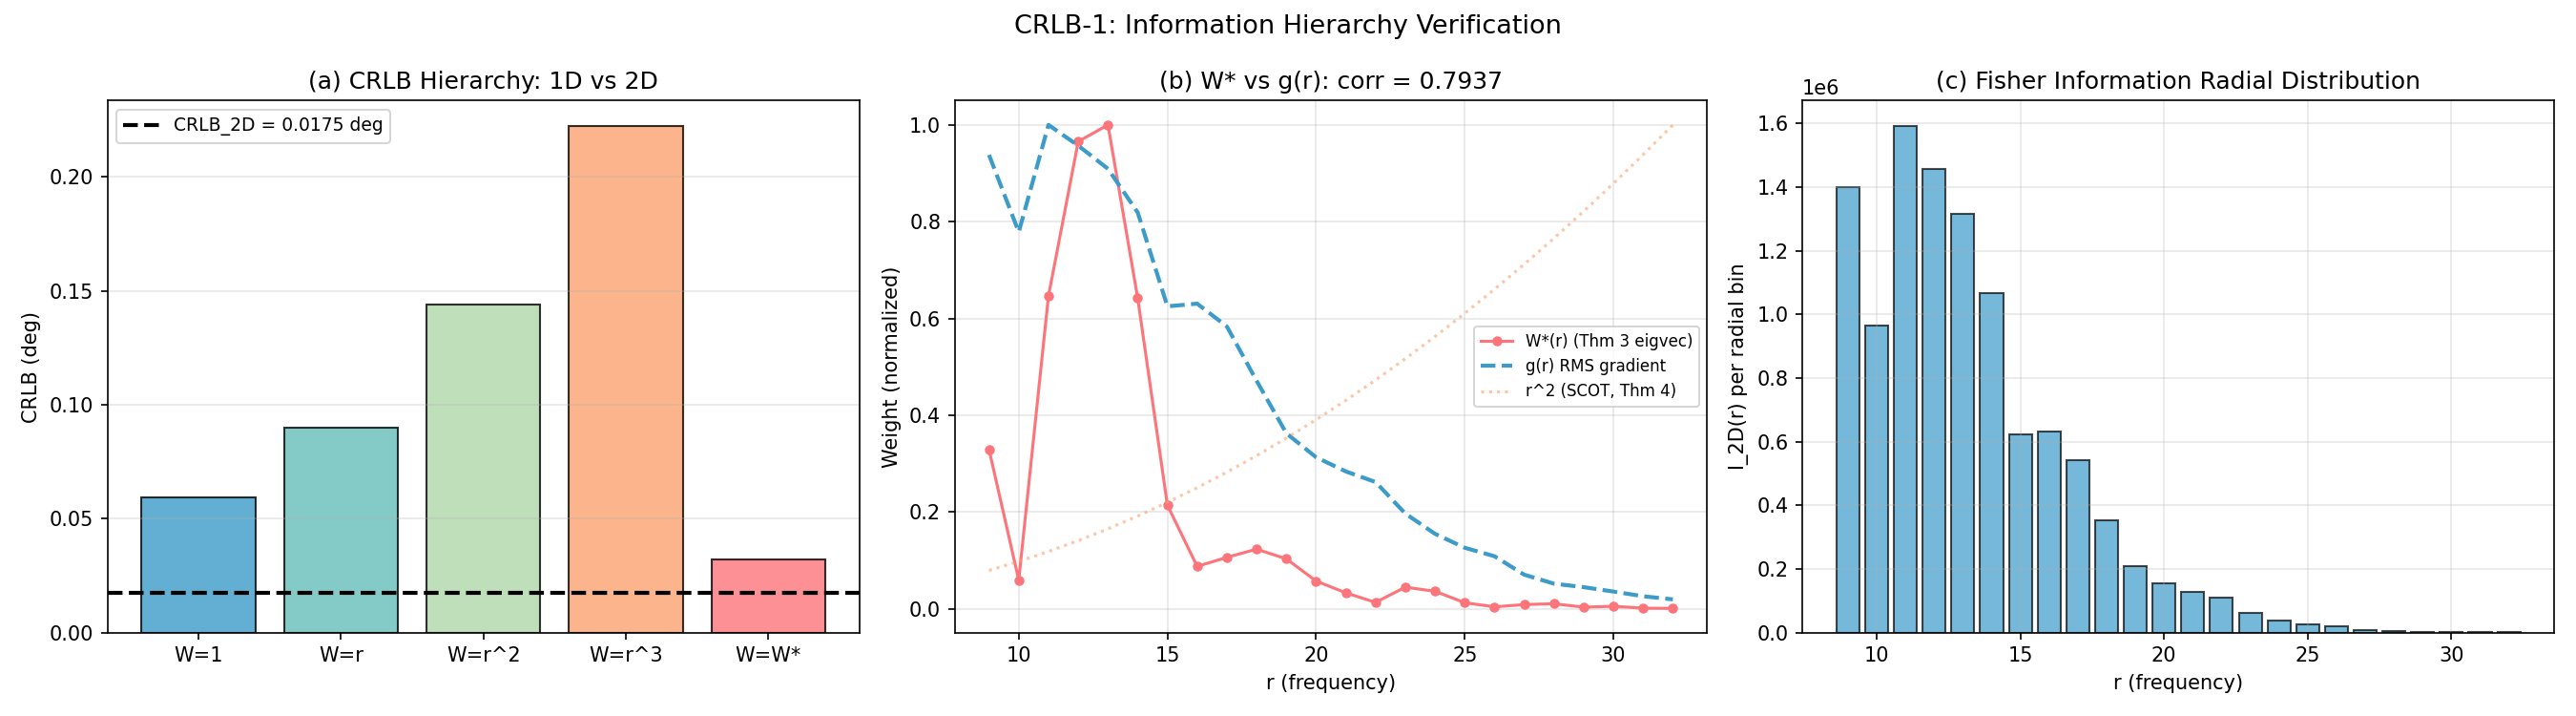
\includegraphics[width=\columnwidth]{figures/main/fig04_crlb_hierarchy.png}
  \caption{Numerical validation of CRLB hierarchy for rotation estimation
    ($\sigma_s=0.01$, $N=64$\,px):
    (a) $\CRLB_{1D}^{1/2}$ under five weighting functions versus $\CRLB_{2D}^{1/2}=0.018^\circ$;
    (b) comparison between optimal $W^*(r)$ and $r^2$ ($r=0.80$);
    (c) radial cumulative Fisher information $\mathcal{I}_{2D}$.}
  \label{fig:crlb1_hierarchy}
\end{figure}
%---

\subsection{Rankine-Vortex Rotation-Rate Estimation Results}

Section~\ref{sec:exp_rotation} has already established the Rankine vortex as the primary validation scenario of the paper
and reported the main comparison result of the final protocol against the gradient baseline.
Because the Rankine setting simultaneously contains finite-window translation, rotational structure, and computable ground truth,
it most clearly exposes the difference between the direct-estimation path and the gradient path.

%--- Fig. 6
\begin{figure}[!b]
  \centering
  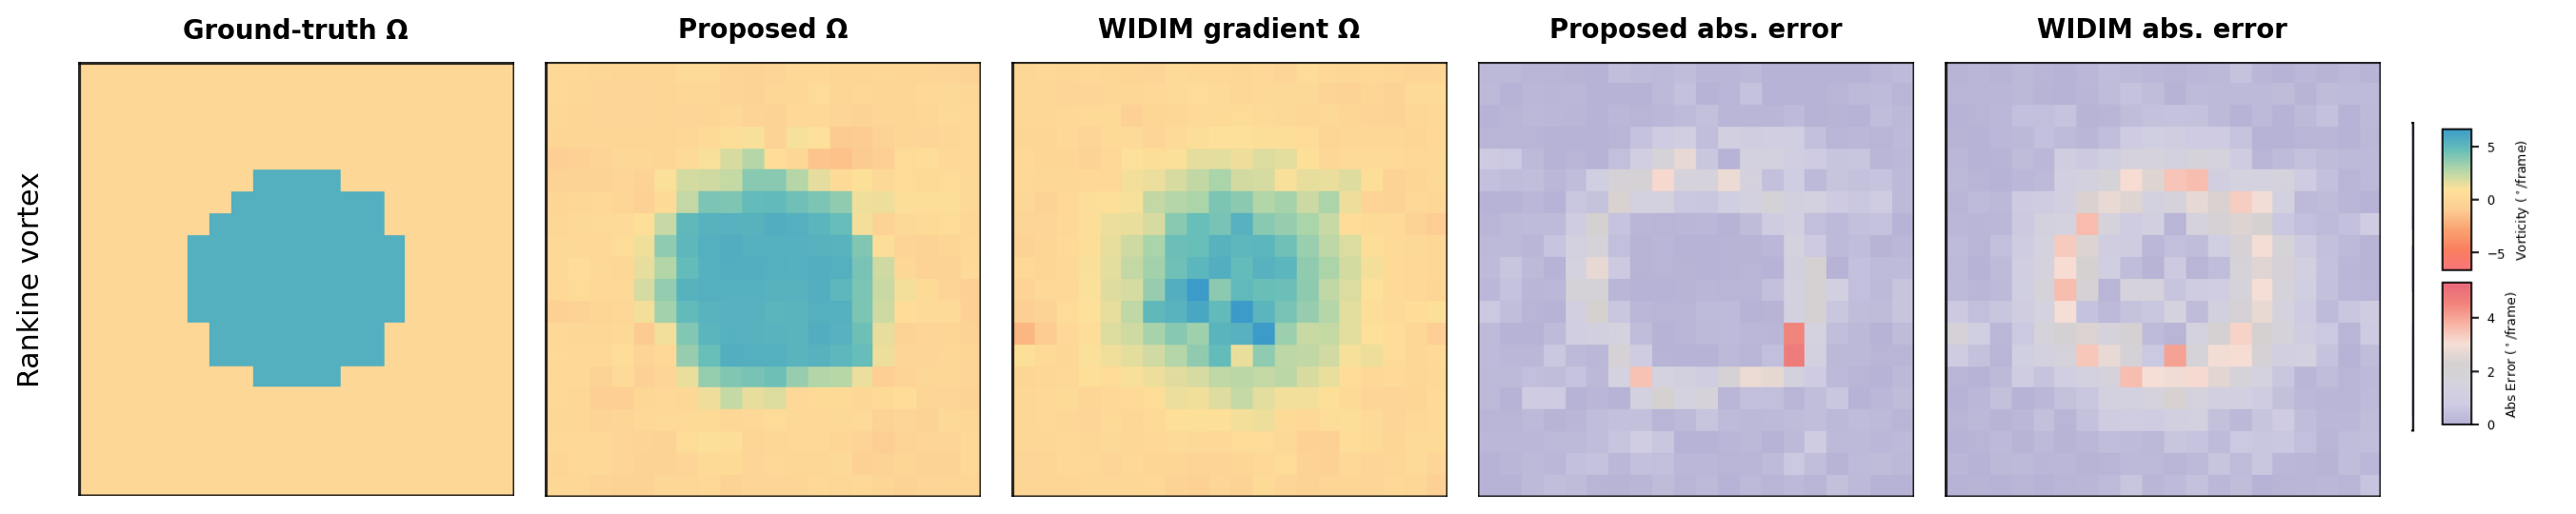
\includegraphics[width=\columnwidth]{figures/main/fig06a_rankine_field.png}
  \caption{Single-seed Rankine visualization under the final track-prior protocol
    ($\sigma_s=0.01$).
    The figure shows the ground-truth rotation-rate field, the proposed field,
    the WIDIM gradient field, and the corresponding absolute-error maps on the same
    $20\times20$ scan grid.}
  \label{fig:rankine_field_vis}
\end{figure}
%---

\begin{figure}[!t]
  \centering
  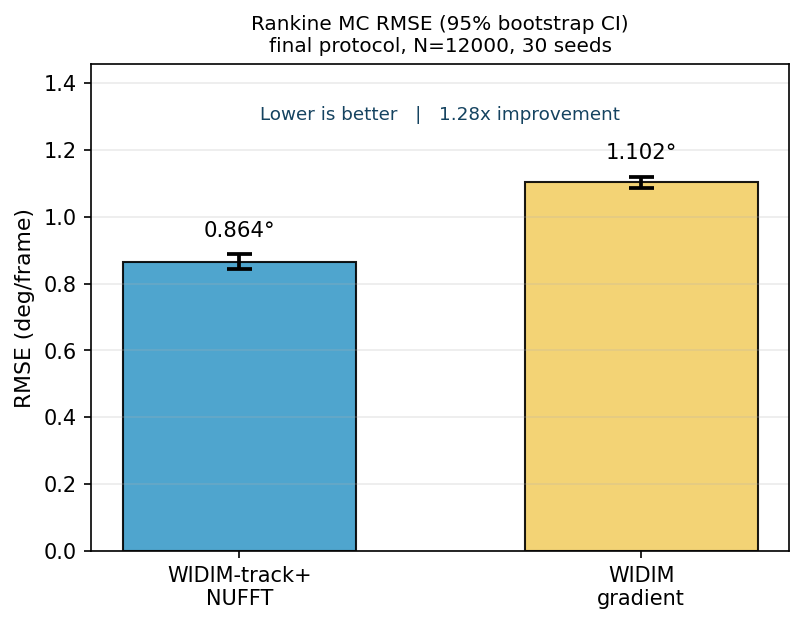
\includegraphics[width=\columnwidth]{figures/main/fig06b_rankine_mc.png}
  \caption{Monte Carlo RMSE summary for the final Rankine protocol
    ($N=12000$, 30 seeds, $\sigma_s=0.01$).
    WIDIM-track+NUFFT ($0.864^\circ$, 95\% CI $[0.842,0.887]$)
    outperforms the WIDIM gradient baseline
    ($1.102^\circ$, 95\% CI $[1.084,1.119]$) by $1.28\times$
    (a $21.6\%$ RMSE reduction). Proxy-to-truth calibration for real-data interpretation is reported separately in Table~\ref{tab:proxy_calibration} and the supplement.}
  \label{fig:rankine_mc}
\end{figure}
%---

\subsection{Multi-Flow Ground-Truth Rotation-Rate Comparison}

% --- Fig. 13 multi-flow ground-truth comparison (two-column)
\begin{figure*}[!t]
  \centering
  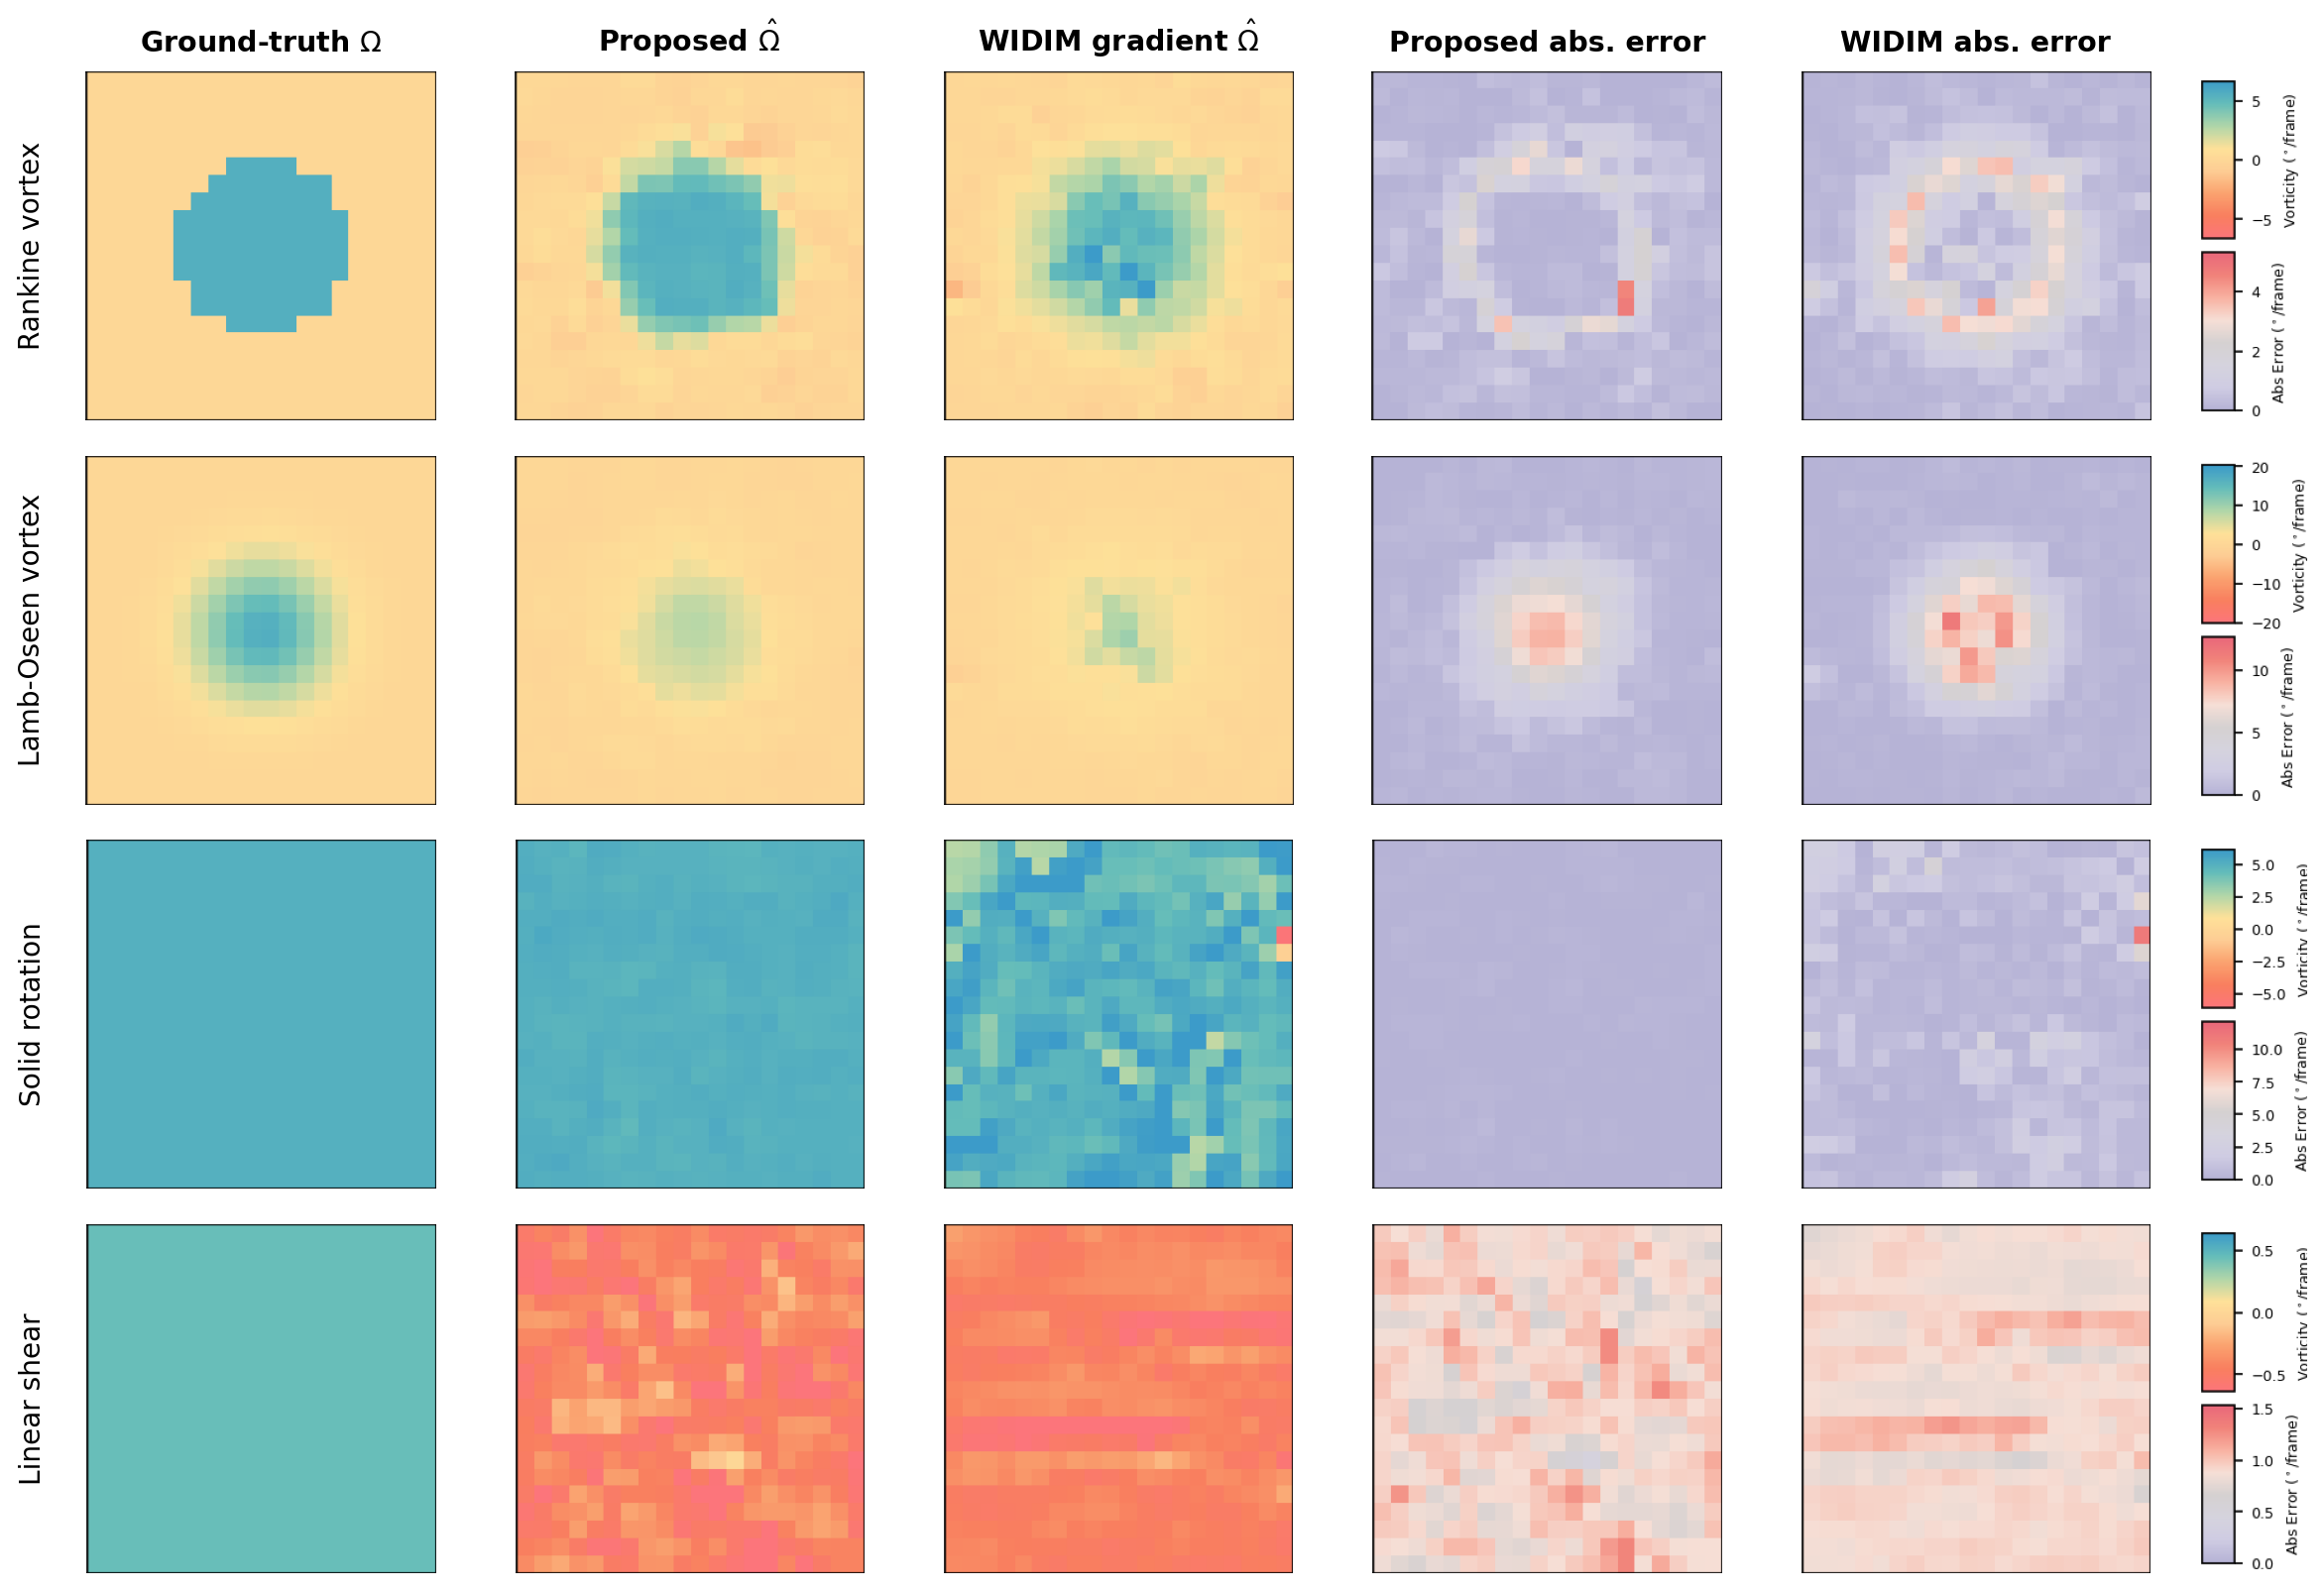
\includegraphics[width=0.96\textwidth]{figures/main/fig07_gt_vorticity.png}
  \caption{Ground-truth rotation-rate comparison across four synthetic flows
    ($\sigma_s=0.01$, seed=42 visualization).
    Columns: analytic truth, NUFFT estimate, WIDIM-gradient estimate, NUFFT absolute error, and WIDIM absolute error.
    Quantitative RMSE values are reported in Table~\ref{tab:gt_vorticity}.}
  \label{fig:gt_vorticity}
\end{figure*}
%---

Section~\ref{sec:exp_gt_vorticity} has already reported the main numerical results on four analytic ground-truth flows.
These scenarios are used here to identify where the direct-estimation advantage remains strong and where it weakens.
Figure~\ref{fig:gt_vorticity} provides flow-by-flow truth and error comparisons,
whereas Fig.~\ref{fig:gt_summary} in the methodology section has already summarized the V0--V3 protocol evolution quantitatively across flows.

\subsection{Near-Real Ground-Truth Bridge}

A near-real ground-truth bridge benchmark is introduced between ideal analytic truth and real data without truth.
It uses the same final protocol and gated evaluation convention as the real-data study while progressively adding particle turnover, particle-density fluctuation, nonuniform illumination, background noise, and weak flow perturbation.
These factors define a four-level realism ladder from L0 (ideal) to L3 (near-real).
Across Rankine, Lamb--Oseen, solid rotation, and a vortex+translation+shear mixed flow, $4\times4\times8=128$ cases are evaluated to test whether the true-accuracy advantage over the WIDIM gradient baseline persists as rendering departs from ideal synthetic conditions.

Figures~\ref{fig:bridge_visual} and~\ref{fig:bridge_truth_realism} report the L3 visualizations and the flow-wise quantitative trends of this bridge layer.
Relative to the ideal Rankine experiment, this benchmark introduces stronger particle loss, illumination fluctuation, and local mismatch, and is substantially closer to real PIV windows.

\begin{figure}[!t]
  \centering
  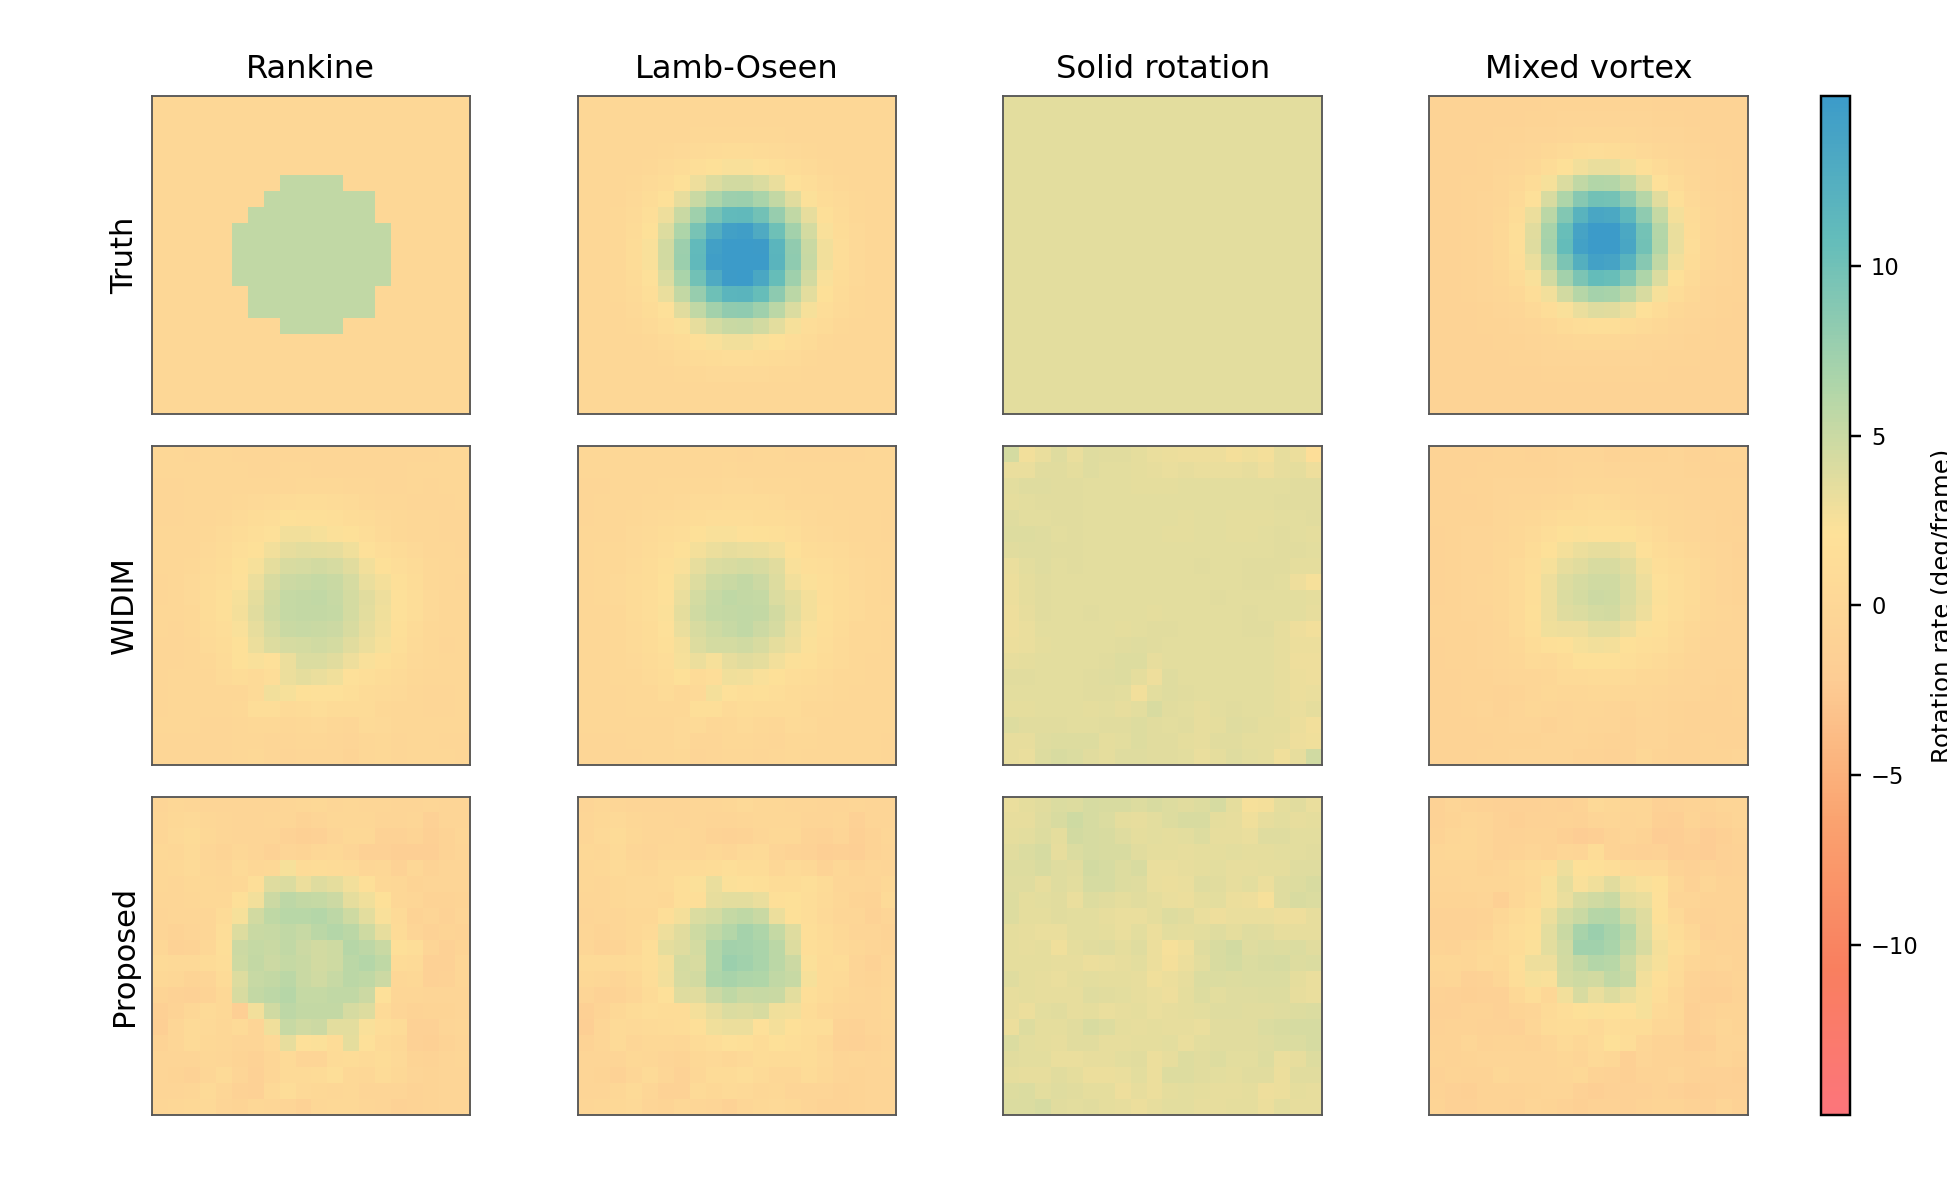
\includegraphics[width=\columnwidth]{figures/main/fig08_bridge_visual.png}
  \caption{Near-real truth bridge visualization at the L3 rendering level.
    Rows: ground-truth field, WIDIM-gradient field, and final proposed field.
    Columns: Rankine, Lamb--Oseen, solid rotation, and mixed vortex.}
  \label{fig:bridge_visual}
\end{figure}

\begin{figure}[!t]
  \centering
  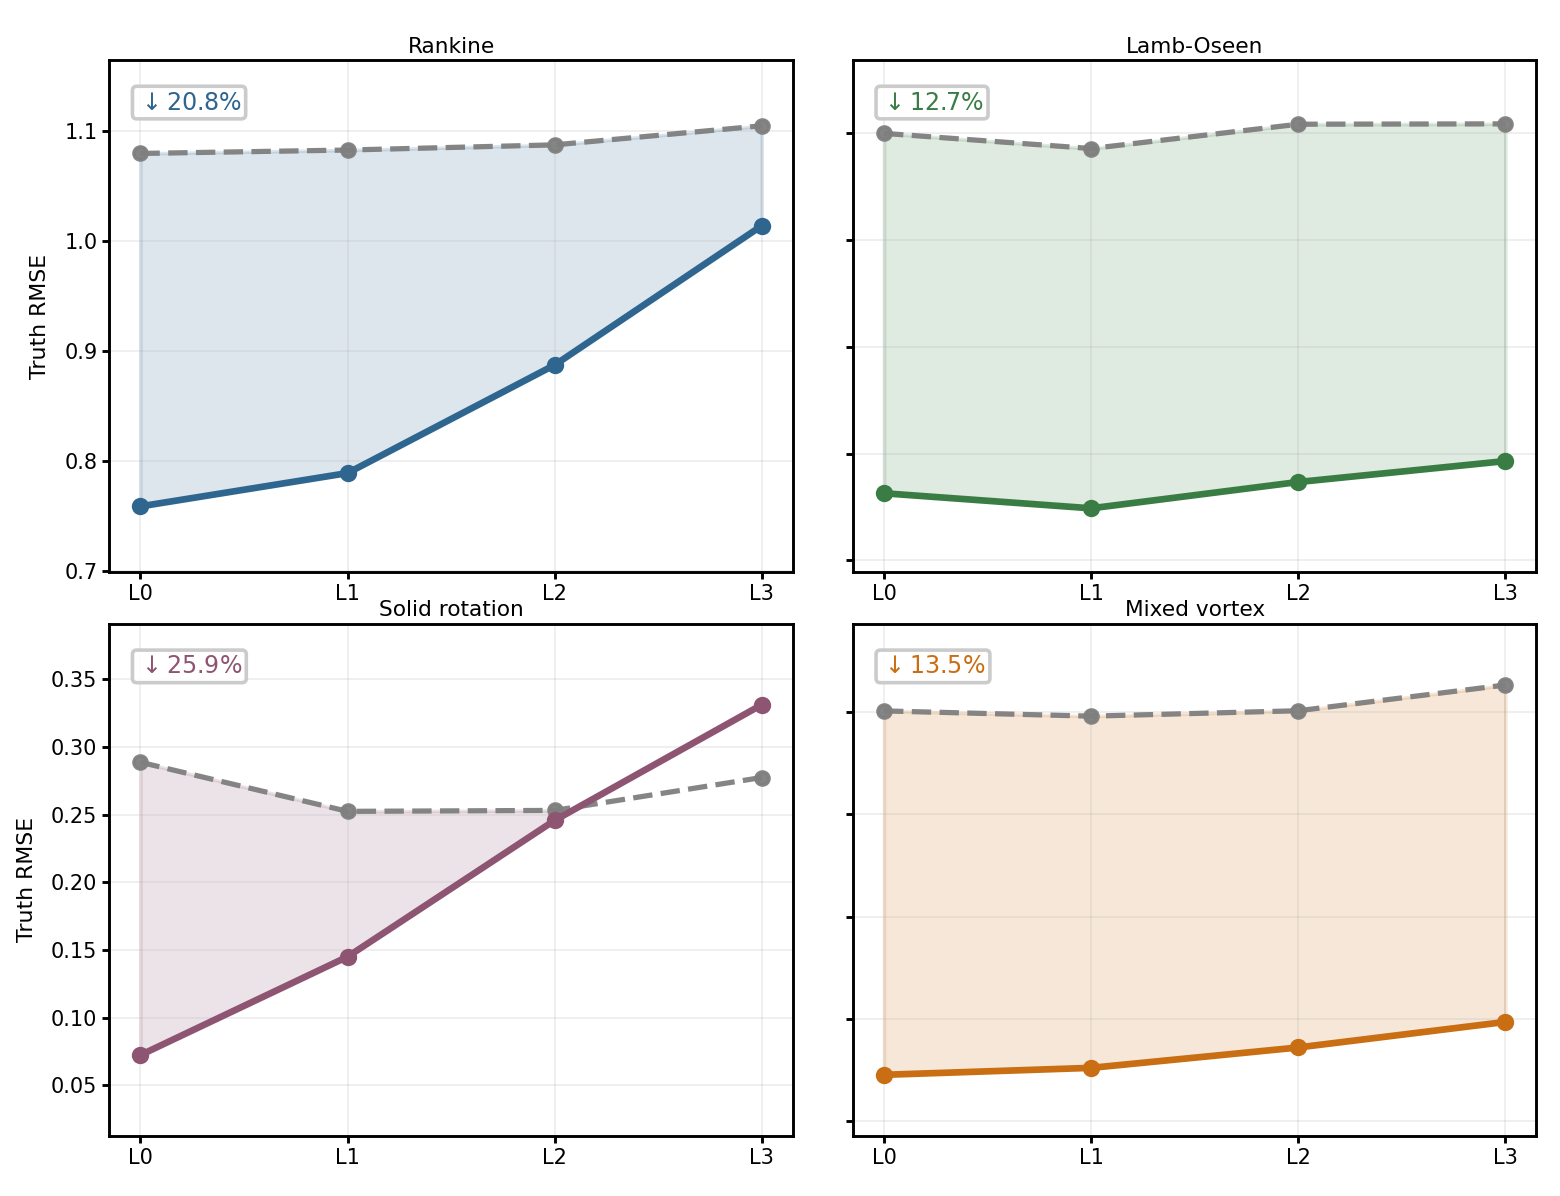
\includegraphics[width=\columnwidth]{figures/main/fig08_bridge_truth_vs_realism.png}
  \caption{Near-real truth bridge benchmark.
    Each panel tracks one bridge flow under increasing realism;
    dashed curves denote WIDIM and solid curves denote the final protocol.}
  \label{fig:bridge_truth_realism}
\end{figure}

In Rankine, Lamb--Oseen, and mixed-vortex settings---all of which contain translation-bearing rotational structure---
the WIDIM field tends to become more diffuse and exhibits weakened peaks,
whereas the final protocol preserves a more concentrated rotational structure.
Solid rotation acts as a control case in this bridge layer because the motion is spatially uniform and leaves relatively little mismatch for the direct path to recover.
The quantitative result is summarized in Fig.~\ref{fig:bridge_truth_realism}.
Across all 128 cases,
the final protocol reduces the ground-truth RMSE from $1.616^\circ/\mathrm{frame}$ to $1.374^\circ/\mathrm{frame}$,
corresponding to an average $15.0\%$ reduction,
and yields positive $\Delta\mathrm{RMSE}_{\mathrm{true}}$ in $114/128$ cases.
When aggregated at the flow-by-level granularity,
$15$ of the $16$ combinations remain positive.
Flow-wise, the mean RMSE decreases by $20.8\%$, $12.7\%$, $25.9\%$, and $13.5\%$
for Rankine, Lamb--Oseen, solid rotation, and mixed vortex, respectively;
only the L3 solid-rotation case exhibits a slight reversal,
consistent with the boundary behavior already seen in the multi-flow synthetic experiment.

\subsection{Real-Data Results and Discussion}

Real-data interpretation relies on two preceding results.
The near-real bridge benchmark establishes a truth-level advantage over WIDIM under more realistic rendering conditions, whereas Table~\ref{tab:proxy_calibration} calibrates the gated proxy gains against raw-to-final truth gains.
The real-data results are treated as calibrated evidence of deployment robustness and structural recovery.

Table~\ref{tab:proxy_calibration} reports the corresponding synthetic calibration under the unified evaluation convention.
Using a separate 20-seed calibration set, $\Delta\mathrm{Corr}_{\mathrm{gate}}$, $\Delta\mathrm{RMSE}_{\mathrm{gate}}$, and $\Delta\mathrm{MAE}_{\mathrm{gate}}$ are mapped to the ground-truth gain $\Delta\mathrm{RMSE}_{\mathrm{true}}$.
The calibration identifies $\Delta\mathrm{RMSE}_{\mathrm{gate}}$ and $\Delta\mathrm{MAE}_{\mathrm{gate}}$ as the most stable proxies, with $\Delta\mathrm{Corr}_{\mathrm{gate}}$ serving as supporting evidence for structural recovery.

\begin{table}[!htbp]
  \renewcommand{\arraystretch}{1.15}
  \caption{Synthetic calibration linking the real-data gated gains to the
    raw-to-final ground-truth RMSE gain
    (separate 20-seed calibration set)}
  \label{tab:proxy_calibration}
  \centering
  \scriptsize
  \setlength{\tabcolsep}{3.2pt}
  \begin{threeparttable}
    \begin{tabular}{@{}lcc@{}}
      \toprule
      Evaluation gain & All synthetic ($N_{\mathrm{cases}}=80$) & Rankine ($N_{\mathrm{cases}}=20$) \\
      \midrule
      $\Delta \mathrm{Corr}_{\mathrm{gate}}$ & $0.963 \,/\, 76.2\%$ & $0.970 \,/\, 95.0\%$ \\
      $\Delta \mathrm{RMSE}_{\mathrm{gate}}$ & $0.994 \,/\, 86.2\%$ & $0.999 \,/\, 95.0\%$ \\
      $\Delta \mathrm{MAE}_{\mathrm{gate}}$ & $0.977 \,/\, 88.8\%$ & $0.962 \,/\, 95.0\%$ \\
      \bottomrule
    \end{tabular}
    \begin{tablenotes}
      \footnotesize
      \item Each cell reports Pearson correlation / sign-agreement rate
            between the reported gain and the raw-to-final
            $\Delta\mathrm{RMSE}_{\mathrm{true}}$.
            Positive $\Delta$ indicates improvement of the final protocol
            over raw NUFFT under the same gated mask.
    \end{tablenotes}
  \end{threeparttable}
\end{table}

Table~\ref{tab:proxy_calibration}, together with the supplement scatter plots, shows that $\Delta\mathrm{RMSE}_{\mathrm{gate}}$ is nearly linearly related to raw-to-final $\Delta\mathrm{RMSE}_{\mathrm{true}}$ and serves as the primary real-data quantity.
By contrast, $\Delta\mathrm{Corr}_{\mathrm{gate}}$ remains directionally consistent with true improvement but is more sensitive to the continuity of the underlying flow structure and is treated only as supporting evidence for structural recovery.
The resulting interpretation has two complementary modes: complex texture, local occlusion, or window mismatch mainly reduce $\Delta\mathrm{RMSE}_{\mathrm{gate}}$ and $\Delta\mathrm{MAE}_{\mathrm{gate}}$, whereas continuous vortex rings or vortex cores more readily yield additional gains in $\Delta\mathrm{Corr}_{\mathrm{gate}}$ and structural coherence~\cite{Shan2025Lightweight,Choi2023SpatialRefinement,Elrefaie2024StereoPIV}.

\subsubsection{Overall Real-Data Results}

Under the calibrated unified protocol, the final method exhibits stable gains over all 320 real PIV image pairs:
the mean $\Delta\mathrm{RMSE}_{\mathrm{gate}}$ is $8.43^\circ/\mathrm{frame}$ ($22.5\%$ reduction), the mean $\Delta\mathrm{MAE}_{\mathrm{gate}}$ is $7.41^\circ/\mathrm{frame}$ ($26.0\%$ reduction), and the mean $\Delta\mathrm{Corr}_{\mathrm{gate}}$ is $0.0068$ ($27.5\%$ increase).
Moreover, $\Delta\mathrm{RMSE}_{\mathrm{gate}}>0$ and $\Delta\mathrm{MAE}_{\mathrm{gate}}>0$ hold for all 320 samples, showing that relative to raw NUFFT, WIDIM(track)+NUFFT+Adaptive p5 Gate consistently suppresses catastrophic local mismatches and produces a more robust rotation-rate field.
Table~\ref{tab:real_proxy_overview} summarizes the pooled statistics,
Fig.~\ref{fig:real_gain_modes} separates the two real-data gain modes of tail suppression and structural recovery,
and Fig.~\ref{fig:real_proxy_case} provides a representative real vortex-ring case.

\begin{figure}[!b]
  \centering
  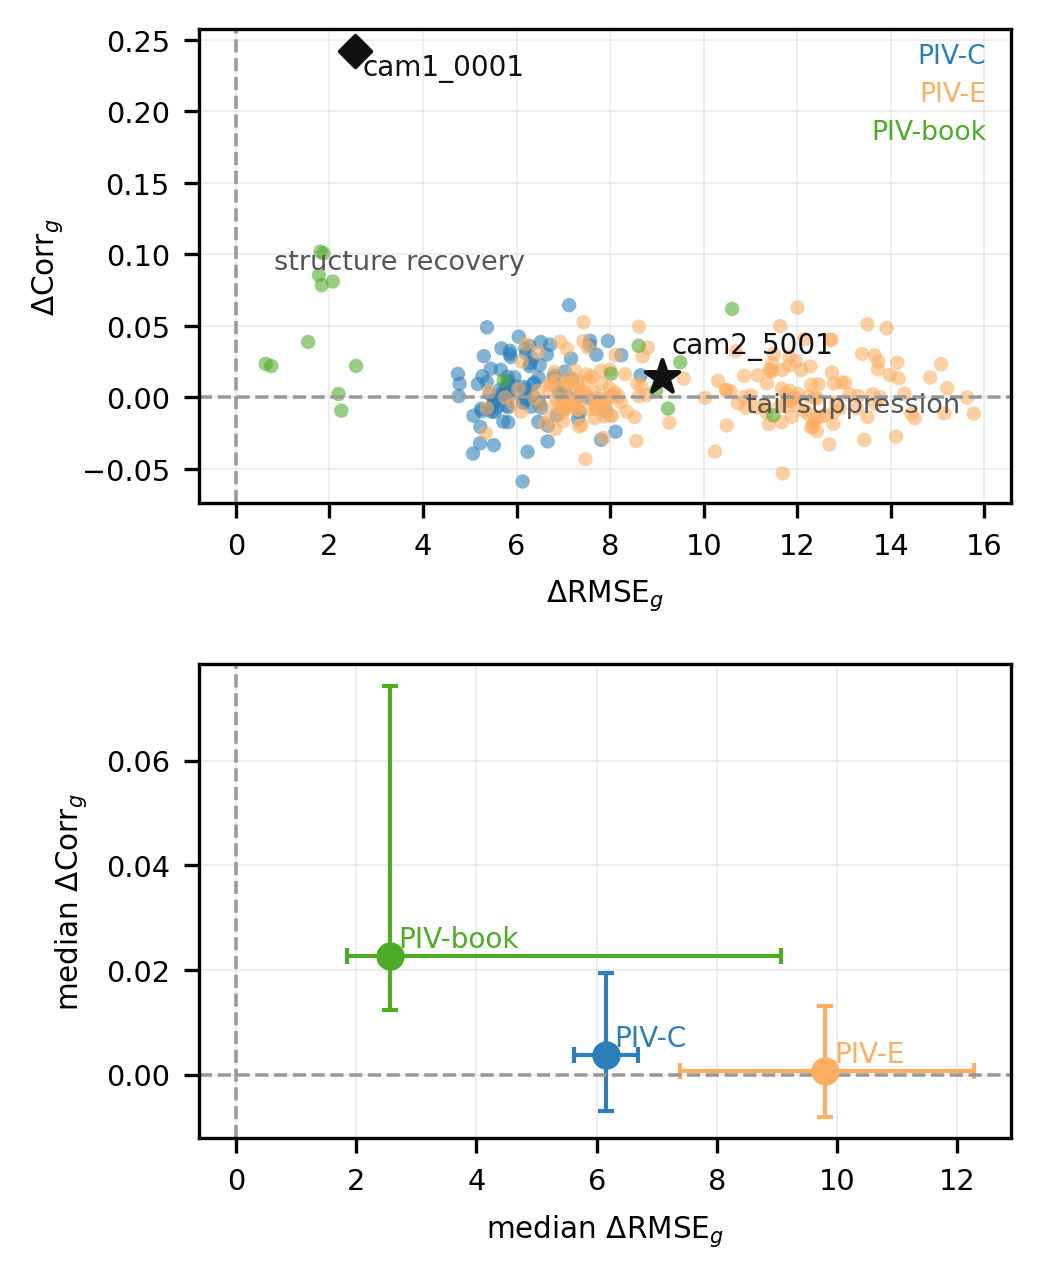
\includegraphics[width=0.76\columnwidth]{figures/main/fig09_real_gain_modes.png}
  \caption{Gain modes on all 320 real PIV pairs.
    Top: pairwise gains in the $\Delta\mathrm{RMSE}_{\mathrm{gate}}$--$\Delta\mathrm{Corr}_{\mathrm{gate}}$ plane.
    Bottom: source medians with interquartile ranges; \texttt{cam2\_5001} marks a simultaneous tail-suppression and structure-recovery case.}
  \label{fig:real_gain_modes}
\end{figure}

Disaggregated by source pool, PIV-E yields the largest $\Delta\mathrm{RMSE}_{\mathrm{gate}}$ and $\Delta\mathrm{MAE}_{\mathrm{gate}}$ (reductions of $19.7\%$ and $24.0\%$, respectively), indicating that the final protocol is particularly effective at compressing large-error tails in visually complex real images.
PIV-book, by contrast, yields the largest $\Delta\mathrm{Corr}_{\mathrm{gate}}=0.0433$ ($148.9\%$ increase), indicating stronger recovery of continuous vortex-ring or vortex-core structure.
Within that subset, cam1 shows the most stable structural recovery, whereas cam2 has the larger $\Delta\mathrm{RMSE}_{\mathrm{gate}}$ and $\Delta\mathrm{MAE}_{\mathrm{gate}}$, which is why the main-text example uses \texttt{cam2\_5001}.
In \texttt{cam2\_5001}, an additional structure-based check that does not use WIDIM as the evaluation target shows that a ring-centered ROI extracted from the gated proposed field achieves higher annulus-to-background contrast (1.34 versus 0.77) and a slightly longer continuous arc than the corresponding WIDIM ROI, supporting better recovery of the visible vortex-ring segment.

\subsection{Scenario Dependence and Influencing Factors on Real Data}

The real-data differences fall into two regimes.
When complex texture, local occlusion, or window mismatch is more pronounced, the gain appears first as reductions in $\Delta\mathrm{RMSE}_{\mathrm{gate}}$ and $\Delta\mathrm{MAE}_{\mathrm{gate}}$.
When continuous vortex-ring or vortex-core structure dominates, it further appears as increased $\Delta\mathrm{Corr}_{\mathrm{gate}}$ and structural recovery.
The governing factors are the spatial continuity of the rotational organization, the concentration of low-confidence windows into patches, and the severity of local mismatch in raw NUFFT.

\subsection{Deployment-Side Gain Mechanism and Discussion Boundary}

Both gain modes arise from the physical coupling between finite-window PIV and the direct estimator.
Particle inflow and outflow weaken local spectral correspondence and induce low-SNR isolated windows, whereas affine de-rotation would remove part of the rotational component to be measured.
The final protocol keeps only a translation-only prior to restore window correspondence and uses Adaptive p5 gating together with two-stage refill to compress the long-tail variance introduced by low-confidence windows.
As a result, complex texture and local mismatch first manifest as decreases in $\Delta\mathrm{RMSE}_{\mathrm{gate}}$ and $\Delta\mathrm{MAE}_{\mathrm{gate}}$, whereas continuous vortex-ring structures further manifest as increases in $\Delta\mathrm{Corr}_{\mathrm{gate}}$ and structural recovery~\cite{Walbecq2024Boundary,Willert2025WSS,Elrefaie2024StereoPIV}.

\FloatBarrier

% ------------------------------------------------------------------
\section{Conclusion}
\label{sec:conclusion}
% ------------------------------------------------------------------

Local rotation-rate measurement in PIV is better posed as direct spectral angular-shift estimation than as a quantity derived from an estimated displacement field.

\begin{enumerate}
  \item \textbf{Theory.}
    A CRLB framework is established that directly targets the local rotation angle and rotation rate and makes the structural precision limitation of the WIDIM gradient path explicit.
    Under the convention $\Omega=\tfrac{1}{2}(\partial v/\partial x-\partial u/\partial y)$,
    the uncertainty propagates from displacement error as $O(\sigma_d/\Delta x)$,
    which cannot be substantially reduced merely by continuing to improve WIDIM peak localization itself.

  \item \textbf{Algorithm.}
    Direct rotation estimation from the NUFFT polar magnitude spectrum reaches about $80\%$ CR efficiency under uniform rotation
    relative to $\CRLB_{1D}=0.144^\circ$.
    In deployable form,
    WIDIM(track)+NUFFT+Adaptive p5 Gate reduces the RMSE in the Rankine scenario
    from $1.102^\circ$ to $0.864^\circ$ ($1.28\times$ improvement, corresponding to a $21.6\%$ reduction, MC $N=12000$),
    remains better than the gradient baseline in translation-bearing rotational synthetic flows,
    and becomes comparable in pure solid-body rotation and linear shear, which act as control cases delimiting the operating regime rather than as the primary localized-vortex targets.

  \item \textbf{Evidence and boundary.}
    The displacement-orthogonality validation shows that the final protocol does not degrade the WIDIM displacement branch
    (the displacement RMSE differs by only $+0.04\%$; see Table~\ref{tab:displacement_orthogonality}).
    Under the synthetically calibrated unified evaluation protocol,
    the 320 real-data pairs yield mean gains of $\Delta\mathrm{RMSE}_{\mathrm{gate}}=8.43^\circ/\mathrm{frame}$ ($22.5\%$ reduction),
    $\Delta\mathrm{MAE}_{\mathrm{gate}}=7.41^\circ/\mathrm{frame}$ ($26.0\%$ reduction),
    and $\Delta\mathrm{Corr}_{\mathrm{gate}}=0.0068$ ($27.5\%$ increase).
    In visually complex images, the gain appears mainly as tail suppression;
    in continuous vortical structures, more clearly as recovery of spatial coherence.
    On the representative vortex-ring case \texttt{cam2\_5001}, an independent ring-centered structure check further shows higher annulus-to-background contrast (1.34 versus 0.77) and a slightly longer continuous arc in the proposed field.
\end{enumerate}

\begin{table*}[!htbp]
  \centering
  \renewcommand{\arraystretch}{1.15}
  \caption{Real-data performance under the unified adaptive-$p_5$ protocol}
  \label{tab:real_proxy_overview}
  \vspace{0.2em}
  \scriptsize
  \setlength{\tabcolsep}{4pt}
  \begin{threeparttable}
    \begin{tabular}{lrrrrr}
      \toprule
      Pool & $N$ pairs & mean $\Delta$RMSE$_{\mathrm{gate}}$ & mean $\Delta$MAE$_{\mathrm{gate}}$ & mean $\Delta$Corr$_{\mathrm{gate}}$ & Pos. $\Delta$RMSE \\
      \midrule
      All real pairs & 320 & 8.43 ($22.5\%\downarrow$) & 7.41 ($26.0\%\downarrow$) & 0.0068 ($27.5\%\uparrow$) & 320/320 \\
      PIV-C & 100 & 6.22 ($38.0\%\downarrow$) & 2.76 ($53.5\%\downarrow$) & 0.0057 ($19.9\%\uparrow$) & 100/100 \\
      PIV-E & 198 & 9.91 ($19.7\%\downarrow$) & 10.15 ($24.0\%\downarrow$) & 0.0032 ($14.7\%\uparrow$) & 198/198 \\
      PIV-book & 22 & 5.10 ($28.4\%\downarrow$) & 3.92 ($36.0\%\downarrow$) & 0.0433 ($148.9\%\uparrow$) & 22/22 \\
      PIV-book (cam1) & 11 & 1.78 ($41.0\%\downarrow$) & 0.86 ($37.5\%\downarrow$) & 0.0726 ($190.5\%\uparrow$) & 11/11 \\
      PIV-book (cam2) & 11 & 8.42 ($26.7\%\downarrow$) & 6.97 ($35.9\%\downarrow$) & 0.0140 ($69.9\%\uparrow$) & 11/11 \\
      \bottomrule
    \end{tabular}
    \begin{tablenotes}
      \footnotesize
      \item Positive $\Delta$ indicates improvement of the final protocol over raw NUFFT under the same adaptive-gated mask.
            Percentages denote relative reduction for RMSE/MAE and relative increase for Corr.
    \end{tablenotes}
  \end{threeparttable}
\end{table*}

\begin{strip}
  \centering
  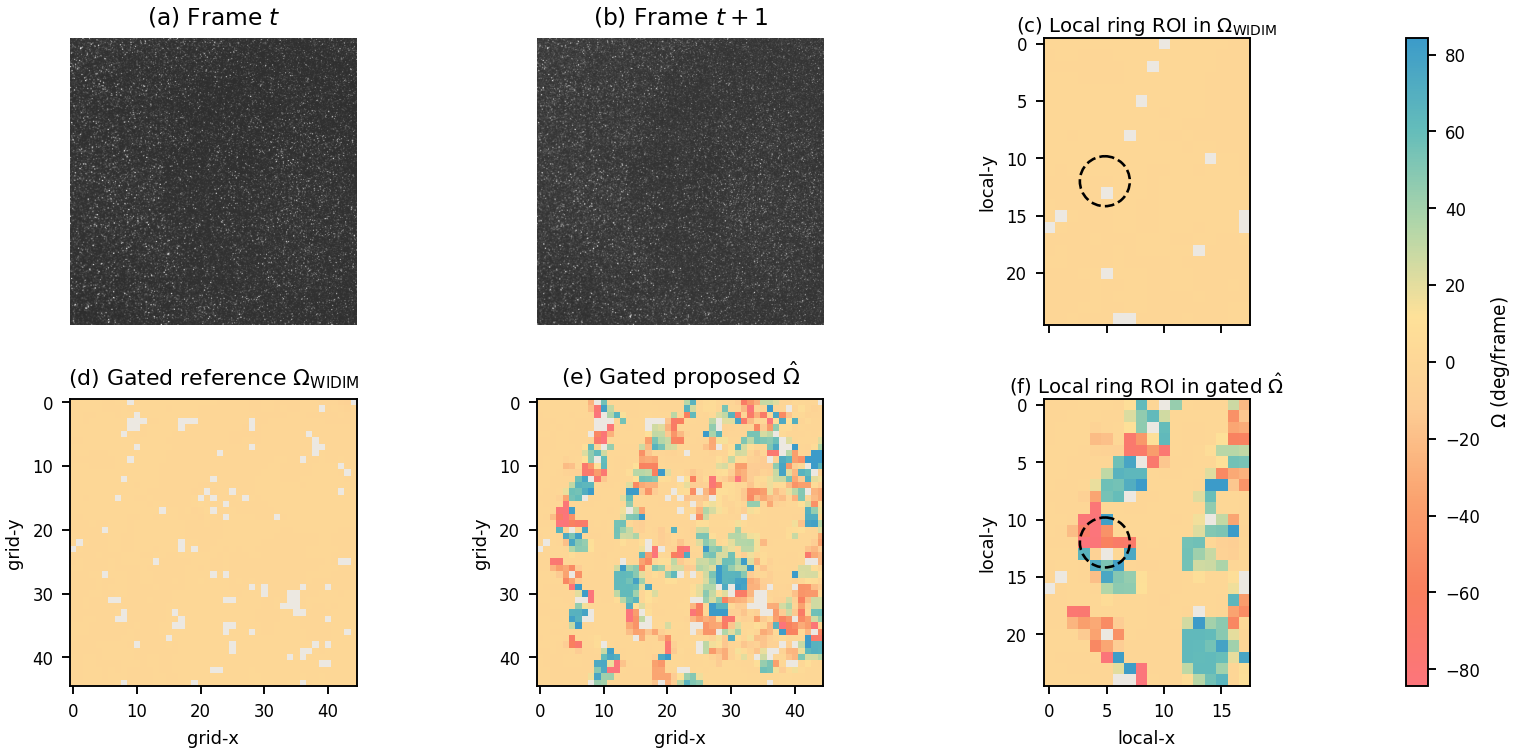
\includegraphics[width=0.90\textwidth]{figures/main/fig10_real_proxy_case.png}
  \captionof{figure}{Real-data evidence of the final WIDIM(track)+NUFFT protocol.
    The representative PIV book \texttt{cam2\_5001} case shows the frame pair, the local ring ROI in the WIDIM and proposed fields, and the corresponding gated full-field maps.
    The dashed circle marks the fitted ring-centered ROI.}
  \label{fig:real_proxy_case}
\end{strip}

% ------------------------------------------------------------------
\section*{Data Availability}
% ------------------------------------------------------------------

The real-data sources used in this manuscript are publicly available from the PIV Challenge website (\url{http://www.pivchallenge.org}; Cases A, C, E, and F) and the PIV book vortex-ring archive (\url{https://pivbook.org}); the single-pair sources (Cases A and F) are merged into the pooled real-data protocol, and the synthetic benchmark cases are generated from standard fluid-dynamics models.

% ──────────────────────────────────────────────────────────────────
%  References
% ------------------------------------------------------------------
\bibliographystyle{IEEEtran}
\bibliography{refs}

\end{document}
